%\documentclass[journal,peerreview,onecolumn]{IEEEtran}
\documentclass[journal]{IEEEtran}
\usepackage{etex}
\usepackage{cite}
\usepackage[pdftex]{graphicx}
\graphicspath{{./Fig/}}
\DeclareGraphicsExtensions{.pdf,.jpg,.png}
\usepackage{amsmath,amssymb,amsthm}
\usepackage{algorithm}
\usepackage{algorithmic}
\usepackage{array}
\usepackage[caption=false,font=footnotesize]{subfig}
\usepackage{fixltx2e}
\usepackage{url}
\usepackage{listings}
\usepackage{multirow}
\usepackage{tikz}
\usepackage{pgfplots}
\usepackage{tabularx}
\usepackage{empheq}
\usepackage{hyperref}
\usepackage{booktabs}
\usepackage{minted}\definecolor{bg}{rgb}{0.95,0.95,0.95}
\newcommand\MyBox[2]{
  \fbox{\lower0.75cm
    \vbox to 1.2cm{\vfil
      \hbox to 1.2cm{\hfil\parbox{1.4cm}{#1\\#2}\hfil}
      \vfil}%
  }%
}

% for peerreview
% \usepackage{setspace}
% \onehalfspacing

\newtheorem{prop}{Proposition}

% correct bad hyphenation here
% \hyphenation{op-tical net-works semi-conduc-tor}

\begin{document}
%
% paper title
% Titles are generally capitalized except for words such as a, an, and, as,
% at, but, by, for, in, nor, of, on, or, the, to and up, which are usually
% not capitalized unless they are the first or last word of the title.
% Linebreaks \\ can be used within to get better formatting as desired.
% Do not put math or special symbols in the title.
\title{Large-scale feature selection with Gaussian mixture models for the classification of high dimensional remote sensing images}
%
%
% author names and IEEE memberships
% note positions of commas and nonbreaking spaces ( ~ ) LaTeX will not break
% a structure at a ~ so this keeps an author's name from being broken across
% two lines.
% use \thanks{} to gain access to the first footnote area
% a separate \thanks must be used for each paragraph as LaTeX2e's \thanks
% was not built to handle multiple paragraphs
%

\author{Adrien~Lagrange,~Mathieu~Fauvel~and~Manuel~Grizonnet% <-this % stops a space
\thanks{A. Lagrange and M. Fauvel are with the Universit\'{e} de Toulouse,
INP-ENSAT, UMR 1201 DYNAFOR, France and with the INRA, UMR 1201
DYNAFOR, France.}%
\thanks{M. Grizonnet is with Centre National d'\'{E}tudes Spatiales, French Space Agency, Toulouse, France.}%
\thanks{This  work was  supported  by the  French National  Research Agency  (ANR)  under  Project Grant  ANR-13-JS02-0005-01  (Asterix project).}}

% The paper headers
\markboth{Transactions on Computational Imaging,~Special Issue on Computational Imaging for Earth Sciences, September~2016}{}

% make the title area
\maketitle

% \tableofcontents
% \clearpage
% As a general rule, do not put math, special symbols or citations
% in the abstract or keywords.
\begin{abstract}
  A  large  scale  feature  selection wrapper  is  discussed  for  the
  classification  of high  dimensional  remote  sensing. An  efficient
  implementation is proposed based on intrinsic properties of Gaussian
  mixtures models and  block matrix.  The criterion  function is split
  into two parts  : one that is  updated to test each  feature and one
  that needs to be updated only once per feature selection. This split
  saved  a  lot  of  computation  for each  test.   The  algorithm  is
  implemented in  \texttt{C++} and integrated into  the Orfeo Toolbox.
  It has been compared to  other classification algorithms on two high
  dimension remote sensing images. The  results show that the approach
  provide good classification accuracies with low computation time.
\end{abstract}

% Note that keywords are not normally used for peerreview papers.
% \begin{IEEEkeywords}
% remote sensing, hyperspectral imaging, feature selection, gaussian mixture model, fast computing.
% \end{IEEEkeywords}

% For peer review papers, you can put extra information on the cover
% page as needed:
% \ifCLASSOPTIONpeerreview
% \begin{center} \bfseries EDICS Category: 3-BBND \end{center}
% \fi
%
% For peerreview papers, this IEEEtran command inserts a page break and
% creates the second title. It will be ignored for other modes.
\IEEEpeerreviewmaketitle

\section{Introduction}
\label{sec:intro}

\IEEEPARstart{W}{ith} the increasing number of remote sensing missions, the quantity of available Earth observation data for a given landscape becomes larger and larger. Satellite missions produce a huge amount of data on a regularly (daily) basis. From 2018, the EnMAP (Environmental Mapping and Analysis Program) satellites managed by the German space agency will produce images with 244 spectral bands, a spatial resolution of 30x30m per pixel and with a frequency of revisit of 4 days\cite{Müller09enmap}. The Hyperspectral Infrared Imager (HyspIRI) of NASA will also deliver images with 212 spectral bands. Additionally to hyperspectral data, the amount of available hypertemporal data increases a lot. For instance, the European satellites Sentinel-2 were launched recently and 2 Terabytes of data will be released every day~\cite{drusch2012sentinel}. The Landsat open archive (\url{http://landsat.usgs.gov/products_data_at_no_charge.php}) has released thousands of images. Such high volume of Earth observation data provides an accurate information of land state and functioning, and helps to improve the understanding of the planet~\cite{rs1010001}. However, processing such data is more and more challenging because of statistical and computational issues.

In the spectral or temporal domain, a pixel is represented by a vector
for   which  each   component  corresponds   to  a   spectral/temporal
measurement.   The size  of  the  vector is  therefore  the number  of
spectral  or temporal  measurements.  For  hyperspectral images,  this
number is  typically about several  hundreds while for  the Sentinel-2
multitemporal images, the number of spectro-temporal measurement for a
given  year  is approximately  one  thousand.   When working  in  high
dimensional  space,  statistical  methods  made for  low  or  moderate
dimensional  space do  not  adapt  well.  For  instance,  the rate  of
convergence of the statistical estimation decreases when the dimension
grows while conjointly the number of parameters to estimate increases,
making    the    estimation    of   the    model    parameters    very
difficult~\cite{donoho}.  Consequently,  with a limited  training set,
beyond a certain limit, the classification accuracy actually decreases
as the number of features increases~\cite{hughes}.  For the purpose of
classification,  these  problems are  related  to  the \emph{curse  of
  dimensionality}. This  is a  major drawback  in many  remote sensing
application since it  is difficult to collect a large  and an accurate
ground-truth.   An intensive  work has  been performed  in the  remote
sensing community  to build accurate classifiers  for high dimensional
images.  Bayesian models~\cite{book:landgrebe}, feature extraction and
feature   reduction   techniques~\cite{book:landgrebe,DR:guided:tour},
random   forest~\cite{1396322},  neural   networks~\cite{5411821}  and
kernel methods~\cite{kernel:methods:rs} have been investigated for the
classification of such images.

The volume of the data is  increasing dramatically with respect to the
number of measurement  per pixel. The data volume  of an hyperspectral
image  is  typically several  hundreds  of  Gigabytes per  acquisition
($\approx$  300km$^2$). Multitemporal  data are  now available  freely
from  internet  stream  (see  for instance  the  Copernicus  data  hub
\url{https://cophub.copernicus.eu/}).  This very  large volume of data
requires   specific   computing  infrastructure.    High   performance
computing   is   actually   investigated   by   the   remote   sensing
community~\cite{christophe2011remote,plaza2011high}.  Main  issues are
related to the use of parallel approach (multi-core, GPU, clusters) to
improve the  processing time, and  to the use of  streaming techniques
when data  does not fit in  memory.  One popular open  source software
solution  is  the Orfeo  Toolbox,  developed  by the  French  National
Agency~\cite{christophe2008orfeo}.   Streaming and  parallel computing
are  conveniently proposed  to the  users/developpers through  several
modules ``\emph{ready to use}''.

A method  to reduce  both statistical and  computational issues  is to
perform a reduction of the dimension. In fact, with the \emph{curse of
  dimensionality}     comes     the      \emph{blessing     of     the
  dimensionality}~\cite{bouveyron2014model}:  high   dimensional  data
space   exhibits  interesting   properties   for  the   classification
purpose.  In  particular,  it  is   possible  to  get  a  parsimonious
representation  of  the  data  while  maintaining  or  increasing  the
classification  accuracy~\cite{jimenez1998supervised}.  For  instance,
in land-cover  classification, given  a set  of spatial,  temporal and
spectral features, it is possible to  extract those which are the most
discriminant      for      the     purpose      of      classification
\cite{fassnacht2014comparison}.   In  hyperspectral   data,  from  the
hundreds of available spectral channels,  it is possible to reduce the
number of channels  to make the processing more efficient  in terms of
statistical complexity  and computational load. In  short, by reducing
the dimension better, classification results is expected with a reduced
computational load.

% Among the various dimension reduction techniques, feature selection demonstrates several appealing for practical situation. The objective of feature selection is to find a subset of the original features with a minimum loss according the objective. Thus, 

% retrieve the most compact representation of the data with minimum loss of information \cite{Guyon:2006:FEF:1208773}. By deleting the redundant information, feature selection allows to reduce dimension and thus avoid statistical issue, increase algorithm speed and limit storage requirements. Moreover, it adds several beneficial side effects. It improves data understanding by identify where is the most relevant information and it is then possible to save resources when organizing a new data acquisition.

There  are  two  main  strategies  to  reduce  dimension~\cite[Chapter
1]{Guyon:2006:FEF:1208773}: features extraction and feature selection.
Feature extraction means reformulate  and summarize the information by
creating new features in combining  the existing ones, it is sometimes
referred to as \emph{feature construction}.  Linear combination of the
initial features  can be extracted using  Principal Component Analysis
(PCA)~\cite{jimenez1998supervised}  or Independent  Component Analysis
\cite{villa2011hyperspectral}.  Supervised extraction  method has also
been investigated  such as Fischer discriminant  analysis and decision
boundary feature  extraction~\cite{book:landgrebe}.  To  the contrary,
features selection  extracts a subset of  existing features identified
as  the most  relevant  by a  given criterion.   This  subset has  the
additional advantage to  be much more understandable  for the end-user
than those constructed by a (non-)linear combination.

Features selection/extraction algorithms can be divided into three classes. The first class is called \emph{filter methods}. They select features independently of the classifier. Features are ranked according to some statistical measures, \emph{e.g.}, correlation or independence. For example,  PCA is a typical unsupervised filter method. Bruzzone \emph{et al.}\cite{bruzzone1995extension} develop a supervised filter method based on Jeffries-Matusita distance to maximize the separability of class distribution. Correlation between bands has been explored for feature selection in hyperspectral data~\cite{demir2008phase}. In general, these methods are fast and do not depend on any classifier. But they do not take into account the properties of the chosen classifier and do not optimize directly the classification accuracy.

The second class are known as \emph{wrapper methods}. They search for the best subset of variables for a given learning model. Since exhaustive searches are too expensive in terms of processing time, several sub-optimal search strategies have been designed, mainly iterative forward or backward search~\cite{whitney1971direct,marill1963effectiveness} or a combination of both~\cite{somol1999adaptive}. The advantage of such methods compare to filter methods is that they are dedicated to a particular model and to a particular learning problem. On the other hand, as they require the training of multiple models to test various set of variables, they are more time consuming.

% The method proposed in this paper is actually a wrapper method which has been optimized in order to accelerate model learning and testing which is the weak point of this family.

The third class corresponds to the \emph{embedded methods}. They do not separate the features selection process from the learning algorithm and allow interaction between the two processes. A popular embedded method is the \emph{Random Forest}. Embedded methods also exist for other models, \emph{e.g.} SVM \cite{guyon2002gene,weston2003use,tuia2015multiclass}.

Despite a large diversity of methods, feature selection algorithms usually do not scale well with the number of pixels to be processed~\cite{fauvel2015fast}. The training computational load is too important to compensate the reduced prediction computational load. Hence, feature selection is not widely used in operational situation. However, methods based on Gaussian Mixture Models (GMM) have several interesting properties that make them suitable for feature selection in the context of large amount of data. By taking advantage of their intrinsic properties, it is possible to increase the computational efficiency with respect to standard implementation.

The contribution of the paper is a forward feature selection method using GMM in continuation of~\cite{fauvel2015fast}. An efficient implementation of the method, using linear algebra on block matrix, is presented in order to handle large amount of data. Furthermore, a floating version of the algorithm is proposed. Several criteria are proposed to handle unbalanced training set.  Finally, the developed algorithm is made available as a remote module of the Orfeo Toolbox~\cite{christophe2008orfeo}.

% Finally, tests are conducted to compare different variations of the method and to compare also to other classifiers (GMM, Random Forest, k-nearest-neighbor) available in the Orfeo Toolbox .

The     remaining    of     the     article     is    organized     as
follows.   Section~\ref{sec:gmm-hd}  presents   GMM  classifiers   and
problems  related to  high-dimensional  feature  spaces. The  features
selection methods are detailed in Section~\ref{sec:selection}. Then an
efficient         implementation        is         presented        in
Section~\ref{sec:implementation}.  Experimental  results on  two  real
high dimensional data-set are given Section~\ref{sec:test}. Conclusion
and perspectives conclude the paper in Section~\ref{sec:conclusion}.

\section{Gaussian Mixture Models in high dimensional spaces}
\label{sec:gmm-hd}

The    following    notations    are   used    in    the    remaining.
$\mathcal{S}  = \{\mathbf{x}_i,y_i\}_{i=1}^{n}$  denotes the  training
set where $\mathbf{x}_i \in \mathbb{R}^d$ is the vector of features of
the  $i^{th}$ sample,  $d$  the number  of spectral/temporal  features,
$y_i = 1,...,C$ the associated label, $C$ the total number of classes,
$n$ the  number of samples  and $n_c$ the  number of samples  of class
$c$.

    \subsection{Gaussian Mixture Models}

    For mixture models, it is assumed  that a given sample $\mathbf{x}$ is
    the realization  of a  random vector which  distribution is  a mixture
    (convex     combination)     of      several     class     conditioned
    distribution~\cite{Fraley00model-basedclustering}:
    \begin{align}
        p(\mathbf{x}) = \sum_{c=1}^{C} \pi_c f_c(\mathbf{x}|\theta)
    \end{align}
    where $\pi_c$ is  the prior, \emph{i.e.}, the  proportion of class
    $c$  and  $f_c$  a  parametric density  function  control by
    $\theta$.

    Among the possible parametric model,  the Gaussian one is the most
    used~\cite{bouveyron2014model}.   It assumes  that each  $f_c$ is,
    conditionally  to  $c$,  a  Gaussian  distribution  of  parameters
    $\boldsymbol{\mu}_c$    and    $\boldsymbol{\Sigma}_c$:
    \begin{multline}
        f_c(\mathbf{x}|\boldsymbol{\mu}_c, \boldsymbol{\Sigma}_c) = \\ \frac{1}{(2\pi)^{\frac{d}{2}} |\boldsymbol{\Sigma}_c|^{\frac{1}{2}}} \exp \left( -\frac{1}{2} (\mathbf{x} - \boldsymbol{\mu}_c)^t \boldsymbol{\Sigma}_c^{-1} (\mathbf{x} - \boldsymbol{\mu}_c) \right).
    \end{multline}

    It  is  referred  to  as  Gaussian  mixture  model  (GMM).   In  a
    supervised    learning    framework,    the    class    parameters
    $\boldsymbol{\mu}_c$,   $\boldsymbol{\Sigma}_c$   and  the   prior
    $\pi_c$ are  usually estimated  through the  conventional unbiased
    empirical estimators:
    \begin{align}
        \hat{\pi}_c &= \frac{n_c}{n},\\
        \hat{\boldsymbol{\mu}}_c &= \frac{1}{n_c} \sum_{\{i|y_i = c\}} \mathbf{x}_i ,\\
        \hat{\boldsymbol{\Sigma}}_c &= \frac{1}{(n_c - 1)} \sum_{\{i|y_i = c\}} (\mathbf{x}_i - \boldsymbol{\mu}_c) (\mathbf{x}_i - \boldsymbol{\mu}_c)^t.
    \end{align}
    To predict the  class of a new unseen sample,  the maximum \emph{a
      posteriori}  rule  is  used:
    \begin{equation*}
        \mathbf{x} \text{ belongs to } c \Leftrightarrow c = \text{arg} \max_{c \in C} p(c) p(\mathbf{x}|c).
    \end{equation*}
    Under the GMM,  and identifying $p(c)$ as $\pi_c$  and $p(\mathbf{x}|c)$ as
    $f_c(\mathbf{x}|\theta)$ and by taking the log, the decision function is obtained
    \begin{eqnarray}\label{eq:decision}
      Q_c(\mathbf{x}) &=& 2 \log \left( p(c) p(\mathbf{x}|c) \right) \nonumber \\
                      &=& - (\mathbf{x} - \boldsymbol{\mu}_c)^t \boldsymbol{\Sigma}_c^{-1} (\mathbf{x} - \boldsymbol{\mu}_c) \nonumber \\
                      & &-\log (|\boldsymbol{\Sigma}_c|) + 2 \log (\pi_c) - d \log (2\pi).
    \end{eqnarray}

    \subsection{Curse of dimensionality in GMM}
    \label{sec:curse:gmm}

    The computation of  eq.~(\ref{eq:decision}) requires the inversion
    of the covariance  matrix and the computation of  the logarithm of
    the determinant.  The  estimation of these terms  suffers from the
    curse of dimensionality\cite{bouveyron2014model}. In practice, the
    number of parameters $\eta_c$ to estimate for each class increases
    quadratically  with   respect  to  the  number   of  features,  as
    illustrated in Figure~\ref{fig:nb-param}.  Hence, if the number of
    observation $n_c$  is small compared  to the number  of parameters
    $\eta_c$, the estimated covariance matrix is badly conditioned and
    thus the computation  of its inverse and its  determinant would be
    unstable.  The  worst situation is  $n_c<\eta_c$ which leads  to a
    singular covariance matrix.  Unfortunately, this situation happens
    regularly in remote sensing.   For instance in hyperspectral image
    classification,  very few  labeled samples  are usually  available
    because of the difficulty and the cost to collect ground-truth.

    \begin{figure}[!t]
        \centering
        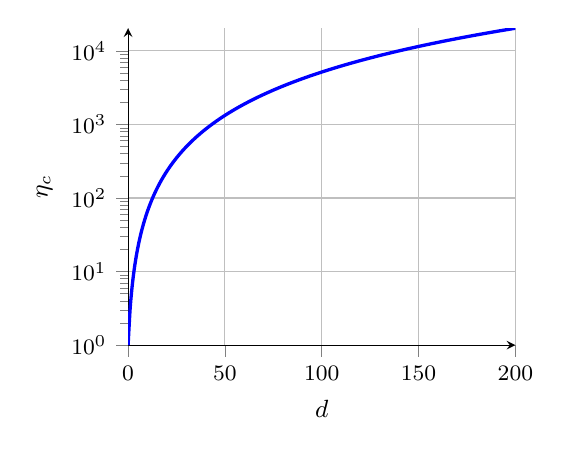
\begin{tikzpicture}
          \begin{axis}[ymode=log,xmin=0,xmax=200,ymin=0,width=0.8\columnwidth,grid,axis x line=left ,axis y line=left, tick align=outside,xlabel = $d$,ylabel = $\eta_c$,small]
            \addplot+[very thick,mark=none,smooth,domain=0:200,samples=200] (\x,{\x*(\x+3)/2+1});
            \end{axis}
        \end{tikzpicture}
        \caption{Number of parameters $\eta_c$ by class in function of dimension $d$: $\eta_c=d(d+3)/2+1$.\label{fig:nb-param}}
    \end{figure}

    There are two major solutions to this problem. First option is to stabilize the inversion of the covariance matrices. Some methods investigate the use of constraints on the direct problem. Reynolds \emph{et al.} \cite{reynolds1995robust} proposed to use diagonal covariance matrices. It is also possible to force the diagonal element to be higher than a given value by maximizing the GMM likelihood \cite{hathaway1985constrained}. Celeux and Govaert \cite{celeux1995gaussian} suggest to use equality constraints between coefficients of the covariance matrix in a parsimonious cluster-based GMM framework. Others papers propose to work on the inverse problem. A classical method is to use a regularization method as the well-known ridge regularization \cite{hoerl1970ridge}. A ridge regularization aims to stabilize the inversion by replacing the covariance matrix $\boldsymbol{\Sigma}_c$ by $\boldsymbol{\Sigma}_c + \tau \mathbf{I}$ where $\tau$ is a positive parameter and $\mathbf{I}$ the identity matrix. Jensen \emph{et al.} \cite{jensen2008regression} propose a different approach using a sparsity approximation to inverse the covariance matrix.

    Second option is to reduce the dimension. Features extraction/selection methods have been developed in order to reduce the dimension with various approaches described in Section~\ref{sec:intro}. In this study, this latter option is explored and a feature selection method named sequential forward features selection is presented.

\section{Sequential forward features selection}
\label{sec:selection}

The feature selection method proposed in this work is a wrapper method associated to GMM models. Two elements are needed to set up a wrapper method:
\begin{enumerate}
\item A function that ranks the features according to some good classification or class separability criteria,
\item A search strategy to optimize the function.
\end{enumerate}

Section~\ref{sec:criterion} describes the different criterion used in this work and two search strategies are discussed in~\ref{sec:selection:method}.


    \subsection{Criterion function}
    \label{sec:criterion}
    The criterion evaluates how a given model built with a subset of features performs for the classification task. It can be an estimation of the correct classification or a measure of separability/similarity between class distribution. The former are in general more demanding in terms of processing time than the later.

    % Criterion functions aim to evaluate either a rate of correct classification or the separability/similarity of class distributions. These functions are used to estimate which sets of variables are the best to represent data, to assure the separability of the classes and to perform classification. The choice of a criterion function is the choice of a way to compare sets of variables.

        \subsubsection{Measures of correct classification}
        \label{sec:criterion-rate}

        A measure of correct classification is based on an error matrix $M$, or \emph{confusion matrix}~\cite[Chapter 4]{congalton2008assessing}. The confusion matrix allows the computation of several global and per-class indices related to the classification accuracy~\cite{congalton2008assessing}. Three global criteria were used in this work:

        \begin{itemize}
        \item  \emph{The overall  accuracy} (OA)  is the  rate of  the
          number of samples with the  correct predicted label over the
          total  number of  samples~\cite{congalton2008assessing}. This
          metric is  easy to interpret  but is  biased in the  case of
          unbalanced classes.

        \item \emph{The Cohen's kappa} (K) is a statistic which measures the probability of agreement between predictions and ground-truth~\cite{congalton2008assessing}.

        \item \emph{The mean F1 score}  (F1mean) is the average of the
          F1 score  for each class  and the  F1 score is  the harmonic
          mean of  the precision  (number of  True Positive  over True
          Positive plus False Positive) and the recall (number of True
          Positive over True Positive plus False Negative)~\cite{powers2011evaluation}.
        \end{itemize}
        High  value  of  theses  indices  correspond  to  an  accurate
        classification.

        These  indices  are  estimated  from the  training  set  by  a
        $n_{cv}$- cross-validation ($n_{cv}$-CV)~\cite{opac-b1127878}.
        To  compute   the  $n_{cv}$-CV,  a  subset   is  removed  from
        $\mathcal{S}$  and  the  GMM  is learned  with  the  remaining
        training samples.  A test error  is computed with  the removed
        training samples  used as validation samples.   The process is
        iterated $n_{cv}$ times and  the estimated classification rate
        is computed as  the mean test error over  the $n_{cv}$ subsets
        of $\mathcal{S}$.

        \hspace{0pt} \\

        \subsubsection{Similarity between distributions}
        The similarity  between two distributions is  quantified using
        divergence  measure~\cite{opac-b1097517}. Contrary  to measure
        of correct  classification, divergences are  computed directly
        on  the  trained  model,  with  no  need  of  cross-validation
        estimation.  Two particular divergences are used in this work:
        the     \emph{Kullback-Leibler}     divergence     and     the
        \emph{Jeffries-Matusita}  distance.   The advantage  of  these
        divergences is  that they have  an explicit expression  in the
        case of Gaussian models. The  simplification allows to get rid
        of  any integration  calculus which  is a  major problem  when
        dealing with high-dimensional data.

        \emph{The   Kullback-Leibler   divergence}   (KL   divergence)
        measures  the  amount  of  information  lost  when  the  first
        distribution     is     approximated     by     the     second
        one\cite{kullback1987letter}. It can be explicitly computed in
        the case of Gaussian distributions:
        \begin{align}
            &KL_{cc^\prime} = \frac{1}{2} \biggl\{ \text{Tr} (\boldsymbol{\Sigma}_c^{-1} \boldsymbol{\Sigma}_{c^\prime}) \nonumber \\
            & + (\boldsymbol{\mu}_c - \boldsymbol{\mu}_{c^\prime})^t \boldsymbol{\Sigma}_c^{-1} (\boldsymbol{\mu}_c - \boldsymbol{\mu}_{c^\prime}) - d + \log \left( \frac{|\boldsymbol{\Sigma}_c|}{|\boldsymbol{\Sigma}_{c^\prime}|} \right) \biggr\},
        \end{align}
        where Tr is the trace operator and $d$ the dimension of the distribution.

        The    KL   divergence    is   not    symmetric,   \emph{i.e.}
        $KL_{cc^\prime} \ne KL_{c^\prime c}$.  A symmetrical version  is used to
        compute the criterion function:
        \begin{align}\label{eq:skl}
          SKL_{cc^\prime} &=KL_{cc^\prime} + KL_{c^\prime c} \nonumber \\
            &= \frac{1}{2} \biggl\{ \text{Tr} (\boldsymbol{\Sigma}_c^{-1} \boldsymbol{\Sigma}_{c^\prime} + \boldsymbol{\Sigma}_{c^\prime}^{-1} \boldsymbol{\Sigma}_c) \nonumber \\
            &~~+ (\boldsymbol{\mu}_c - \boldsymbol{\mu}_{c^\prime})^t (\boldsymbol{\Sigma}_c^{-1} + \boldsymbol{\Sigma}_{c^\prime}^{-1}) (\boldsymbol{\mu}_c - \boldsymbol{\mu}_{c^\prime}) - 2d \biggr\}.
        \end{align}

        The extension  to the multiclass  problem is done  by taking
        the weighted mean  of the KL divergences computed  on all pair
        of classes~\cite{bruzzone1995extension}:
        \begin{equation}
            C_{SKL} = \sum_{c=1}^{C} \sum_{c^\prime = c + 1}^{C} \pi_c \pi_{c^\prime} SKL_{cc^\prime}.
        \end{equation}

        \emph{The Bhattacharyya distance} is defined in the case of Gaussian model as
        \begin{align}
            {B}_{cc^\prime} = &\frac{1}{8} (\boldsymbol{\mu}_c - \boldsymbol{\mu}_{c^\prime})^t \left( \frac{\boldsymbol{\Sigma}_c + \boldsymbol{\Sigma}_{c^\prime}}{2} \right)^{-1} (\boldsymbol{\mu}_c - \boldsymbol{\mu}_{c^\prime}) \nonumber \\
            &+ \frac{1}{2} \log \left( \frac{|\boldsymbol{\Sigma}_c + \boldsymbol{\Sigma}_{c^\prime}|}{\sqrt{|\boldsymbol{\Sigma}_c| |\boldsymbol{\Sigma}_{c^\prime}|}} \right).
        \end{align}

        The \emph{Jeffries-Matusita distance} is a measure based on the Bhattacharyya distance. It saturates if the separability between the two distributions increases~\cite{bruzzone2009novel}. The JM distance is defined as
        \begin{equation}\label{eq:jm}
            {JM}_{cc^\prime} = \sqrt{ 2 \{1 - \text{exp}(-B_{cc^\prime})\} }.
        \end{equation}

        Similar to the KL divergence,  a weighted mean of the distance
        between two classes is computed to aggregate the measures in a
        single value:
        \begin{equation}
            {C}_{JM} = \sum_{c=1}^{C} \sum_{c^{\prime} = c + 1}^{C} \pi_c \pi_{c^\prime} {JM}_{cc^\prime}.
        \end{equation}

        \vspace{10 mm}

        % According to \cite{bruzzone2009novel}, it is interesting to notice that the KL divergence increases quadratically with respect to the distance between the mean vectors of the class distributions whereas the measures of correct classification asymptotically tends to one when distributions are perfectly separable. On the contrary, the JM distance tends to saturate as the measures of correct classification.

        Table~\ref{tab:crit} summarizes the presented criterion functions and their characteristics. In the following $J$ denotes one criterion from Table~\ref{tab:crit}.

        \begin{table}[!t]
            \centering
            \caption{Summary of the different criterion functions.\label{tab:crit}}
            \begin{tabular}[b]{lcc}
              \toprule
              Criterion & Type & Complexity \\
              \midrule
              Overall accuracy            & Accuracy   & High \\
              Cohen's kappa               & Accuracy   & High\\
              F1 mean                     & Accuracy   & High\\
              \midrule
              Kullback-Leibler divergences & Divergence & Low \\
              Jeffries-Matusita distance  & Divergence & Low \\
              \bottomrule
            \end{tabular}
        \end{table}

        \subsection{Selection method}
        \label{sec:selection:method}
        Two  sequential  search  algorithms have been  implemented  in  this
        work~\cite{Guyon:2006:FEF:1208773}:  the   sequential  forward
        selection and the sequential  floating forward.  The later one
        is  an   extension  of   the  former.  Both   select  features
        iteratively.

        \subsubsection{Sequential forward features selection}
        \label{sec:forward-presentation}

        The Sequential Forward Selection (SFS) starts with an empty set of selected features.  At each  step, the feature associated to the highest criterion function $J$  is added  to the set. This feature is definitively added to the pool of selected features and the algorithm stops when a given number of variables \emph{maxVarNb} has been reached. The Algorithm~\ref{alg:sfs} presents the process in details.

        \begin{algorithm}
        \caption{Sequential forward features selection\label{alg:sfs}}
        {\footnotesize
        \begin{algorithmic}[1]
        \REQUIRE $\Omega,J,\text{maxVarNb}$
        \STATE $\Omega=\emptyset$
        \STATE $F=\text{\{all variables $f_i$\}}$
        \WHILE{$\text{card}(\Omega) < maxVarNb$}
        \FORALL{$f_i \in F$}
        \STATE $R_i = J(\{\Omega + f_i\})$
        \ENDFOR
        \STATE $j=\text{arg} \max_{i} R_i$
        \STATE $\Omega = \{\Omega + f_j\}$
        \STATE $F = F \setminus f_j$
        \ENDWHILE
        \RETURN $\Omega$
        \end{algorithmic}
        }
        \end{algorithm}

        \subsubsection{Sequential floating forward feature selection}
        \label{sec:floating-presentation}

        The Sequential Floating Forward Selection (SFFS)\cite{somol1999adaptive} is based on two algorithms: the SFS described above and the Sequential Backward Selection (SBS). The SBS is the backward equivalent of SFS. The difference is that it starts with every features in the pool of selected features and tries at each step to remove the less significant one in term of the given criterion function.

        The SFFS works as the SFS but between each step of the SFS algorithm, a backward selection is operated to identify the less important feature. If the criterion value is higher than the best value ever obtained with a set of same size, the identified feature is picked out. The SBS step is repeated while removing the less important feature leads to an increase of the criterion value. Then SFS is called again. The algorithm stops when a given number of features \emph{maxVarNb} has been selected. The Algorithm~\ref{alg:sffs} provides details about the process.

        This SFFS algorithm evaluates more solutions than the SFS algorithm. The results are expected to be better but the trade-off is an increased computational time which is dependent on the complexity of the dataset.

        \begin{algorithm}
        \caption{Sequential floating forward features selection\label{alg:sffs}}
        {\footnotesize
        \begin{algorithmic}[1]
        \REQUIRE $J,\text{maxVarNb}$
        \STATE $\Omega=\overbrace{(\emptyset,...,\emptyset)}^{maxVarNb}$
        \STATE $F=\text{\{all variables $f_i$\}}$
        \STATE $k=0$
        \WHILE{$k < \text{maxVarNb}$}
        \FORALL{$f_i \in F$}
        \STATE $R_i = J(\{\Omega_k + f_i\})$
        \ENDFOR
        \STATE $j=\text{arg} \max_{i} R_i$
        \STATE $k=k+1$
        \IF{$R_j \geq J(\Omega_k)$}
        \STATE $\Omega_k = \{\Omega_{k-1} + f_j\}$
        \STATE $\text{flag}=1$
        \WHILE{$k > 2 \text{ and } \text{flag}=1$}
        \FORALL{$f_i \in \Omega_k$}
        \STATE $R_i = J(\{\Omega_k \setminus f_i\})$
        \ENDFOR
        \STATE $j=\text{arg} \max_{i} R_i$
        \IF{$R_j > J(\Omega_{k-1})$}
        \STATE $\Omega_{k-1} = \{\Omega_k \setminus f_j\}$
        \STATE $k=k-1$
        \ELSE
        \STATE $\text{flag}=0$
        \ENDIF
        \ENDWHILE
        \ENDIF
        \ENDWHILE
        \RETURN $\Omega_{\text{maxVarNb}}$
        \end{algorithmic}
        }
        \end{algorithm}


\section{Efficient implementation}
\label{sec:implementation}
The most  demanding part  of the  algorithm is  the evaluation  of the
criterion  for  all   the  remaining  variables  (see   lines  5-7  in
Algorithm~\ref{alg:sfs}). Calculus are based on linear algebra, and the
numerical  complexity is  on average  $O(d^3)$.  Furthermore,  for the
\emph{accuracy}-type  criterion the  complexity  is  augmented by  the
cross-validation procedure.

An efficient implementation of  the criterion optimization is detailed
in  the following.   It  is  based on  the  symmetry  property of  the
covariance matrix  and block inverse  formula~\cite{IMM2012-03274}.  It is shown  that the criterion  can be split  into two
parts: one that needs to be computed for each tested variable, and one
that  needs to  be  computed only  once per  selection  step. For  the
cross-validation part,  updates rules  are given to  derive sub-models
without the necessity to learn a GMM models for each fold.

\subsection{Statistical update rules}
        \subsubsection{Update for cross validation}
        \label{sec:update-cv}
        Based on \cite{fauvel2015fast}, a method to accelerate the $n_{cv}$-fold cross-validation process in the case of criterion functions based on correct classification measures was implemented. The idea is to estimate the GMM with the whole training set once and then, instead of training models on $(n_{cv}-1)$ folds, parameters of the complete model are used to derive those of sub-models, thus reducing the whole complexity.

        \begin{prop}[Mean update for cross-validation]
            \label{eq:update-cv1}
            \begin{equation*}
                \boldsymbol{\hat{\mu}}_c^{n_c-\nu_c} = \frac{n_c \boldsymbol{\hat{\mu}}_c^{n_c} - \nu_c \boldsymbol{\hat{\mu}}_c^{\nu_c}}{n_c - \nu_c} \nonumber
            \end{equation*}
        \end{prop}
        \begin{prop}[Covariance matrix update cross-validation]
            \label{eq:update-cv2}
            \begin{align*}
              \boldsymbol{\hat{\Sigma}}_c^{n_c-\nu_c} = &\frac{1}{n_c-\nu_c-1} \biggl\{ (n_c-1) \boldsymbol{\hat{\Sigma}}_c^{n_c} - (\nu_c-1)\boldsymbol{\hat{\Sigma}}_c^{\nu_c} \nonumber \\
                                                        &- \frac{n_c \nu_c}{(n_c-\nu_c)} (\boldsymbol{\hat{\mu}}_c^{\nu_c}-\boldsymbol{\hat{\mu}}_c^{n_c})(\boldsymbol{\hat{\mu}}_c^{\nu_c}-\boldsymbol{\hat{\mu}}_c^{n_c})^t \biggr\} \nonumber
            \end{align*}
        \end{prop}
        \noindent where $n_c$ is the number of samples of class $c$, $\nu_c$ is the number of samples of class $c$ removed from the initial set, exponents on $\boldsymbol{\Sigma}_c$ and $\boldsymbol{\nu}_c$ denotes the set of samples used to compute them.

        \subsubsection{Criterion function computation}
        \label{sec:update-crit}
        At iteration $k$, depending on the criterion, three terms have
        to  be computed:  the inverse  of the  covariance matrix,  the
        logarithm of the determinant of  the covariance matrix and the
        quadratic term in  eq.~(\ref{eq:decision}). However, all these
        terms  have already  been computed  for iteration  $(k-1)$. By
        using the  positive definiteness of the  the covariance matrix
        and block formulae~\cite[Chapter 9.2]{webb2003statistical}, it
        is possible to factorize these terms at iteration $k$.

        In the remaining of the paper, $\boldsymbol{\Sigma}_c^{(k-1)}$
        denotes the  covariance matrix of the  $(k-1)^{th}$ iteration,
        \emph{i.e.}, the  covariance matrix  of the  selected features
        and $\boldsymbol{\Sigma}_c^{(k)}$ denotes  a covariance matrix
        at the $k^{th}$ iteration,  \emph{i.e.}, the covariance matrix
        of  an  augmented  set  by  the  feature  $x_k$.  Then,  since
        $\boldsymbol{\Sigma}_c^{(k)}$ is a positive definite symmetric
        matrix, the covariance matrix can be written as

        % Then, the inverse of  the covariance matrix
        % $(\boldsymbol{\Sigma}^{(k)})^{-1}$,   the   quadratical   term
        % $(\mathbf{x}^{(k)})^t         (\boldsymbol{\Sigma}^{(k)})^{-1}
        % \mathbf{x}^{(k)}$        and        the        log-determinant
        % $\log   |\boldsymbol{\Sigma}^{(k)}|$  can   be  expressed   in
        % function of terms of the $(k-1)^{th}$ iteration.

        \begin{equation}\label{eq:cov}
            \boldsymbol{\Sigma}_c^{(k)} =
            \bigg[\begin{array}{cc}
            \boldsymbol{\Sigma}^{(k-1)}_c & \mathbf{u}_c      \\
            \mathbf{u}_c^t          & \sigma^{(k)}_c \\
            \end{array}\bigg],
        \end{equation}
        where  $\sigma^{(k)}_c$  is  the variance  of  $x_c$,
        $\mathbf{u}_c$ is  the $k^{th}$  column of the  matrix without
        the          diagonal           element,          \emph{i.e.},
        $\mathbf{u}_{c}(i) =  \boldsymbol{\Sigma}^{(k)}_{c}(i,k)$ with
        $i  \in [1,k-1]$.   Using block  matrix inverse  formulae, the
        inverse of  the covariance  matrix is  given by  the following
        proposition.
        \begin{prop}[Forward update rule for the inverse of the covariance matrix]
        \label{eq:update-inv}
        \begin{equation}\label{eq:cov:inv}
                (\boldsymbol{\Sigma}_c^{(k)})^{-1} =
                \bigg[\begin{array}{cc}
                \mathbf{A}_c & \mathbf{v}_c \\
                \mathbf{v}_c^t  & \frac{1}{\alpha_c} \\
                \end{array}\bigg]
            \end{equation}
        \end{prop}
        \noindent                                                where
        $\mathbf{A}_c     =     (\boldsymbol{\Sigma}^{(k-1)}_c)^{-1}     +
        \frac{1}{\alpha_c} (\boldsymbol{\Sigma}^{(k-1)}_c)^{-1} \mathbf{u}_c
        \mathbf{u}_c^t              (\boldsymbol{\Sigma}^{(k-1)}_c)^{-1}$,
        $\mathbf{v}_c           =           -           \frac{1}{\alpha_c}
        (\boldsymbol{\Sigma}^{(k-1)}_c)^{-1}       \mathbf{u}_c$       and
        $      \alpha_c      =      \sigma^{(k)}_c      -      \mathbf{u}_c^t
        (\boldsymbol{\Sigma}^{(k-1)}_c)^{-1}  \mathbf{u}_c$.  This  update
        formulae      is     used      to      obtain     all      the
        $(\boldsymbol{\Sigma}^{(k)}_c)^{-1}$  corresponding  to all  the
        possible augmented set of a given selection iteration. Similar
        update formulae can be written for the backward step.

        % In the case of a backward step in SFFS algorithm, the formula is inverted in order to compute $(\boldsymbol{\Sigma}^{(k-1)})^{-1}$ knowing $(\boldsymbol{\Sigma}^{(k)})^{-1}$. The update rule becomes (proof in Appendix~\ref{app:proof-update})
        % \begin{prop}[Backward update rule for inverse of covariance matrix]
        % \label{eq:update-inv-back}
        %     \begin{equation*}
        %         (\boldsymbol{\Sigma}^{(k-1)})^{-1} = \underbrace{\mathbf{A}}_{\substack{\text{computed once}\\ \text{per selection step}}} - \underbrace{\alpha \mathbf{v} \mathbf{v}^t}_{\substack{\text{computed for} \\ \text{each augmented set}}}
        %     \end{equation*}
        % \end{prop}

        Using eq.~(\ref{eq:cov}) and~(\ref{eq:cov:inv}), it is possible to
        deduce  the   following  propositions  (proof  are   given  in
        Appendix~\ref{app:proof-update}).
        \begin{prop}[Update rule for the quadratical term]
        \label{eq:update-quad}
            \begin{align}
              (\mathbf{x}^{(k)})^t (\boldsymbol{\Sigma}^{(k)}_c)^{-1} \mathbf{x}^{(k)} = &\underbrace{(\mathbf{x}^{(k-1)})^t (\boldsymbol{\Sigma}^{(k-1)}_c)^{-1} \mathbf{x}^{(k-1)}}_{\substack{\text{computed once per selection step}}} \nonumber \\
                                                                                       &+ \underbrace{\alpha_c ( \left[\begin{array}{cc} \mathbf{v}_c^t & \frac{1}{\alpha_c} \end{array}\right] \mathbf{x}^{(k)} )^2}_{\substack{\text{computed for each augmented set}}}.
            \end{align}
        \end{prop}
        \begin{prop}[Update rule for logdet]
        \label{eq:update-log}
            \begin{equation}
                \log \left(|\boldsymbol{\Sigma}^{(k)}_c|\right) = \underbrace{\log \left(|\boldsymbol{\Sigma}^{(k-1)}_c|\right)}_{\substack{\text{computed once}\\ \text{per selection step}}} + \underbrace{\log \alpha_c}_{\substack{\text{computed for} \\ \text{each augmented set}}}.
            \end{equation}
        \end{prop}

        From these update rules, it is now possible to split each criterion into two parts: one computed once per selection step and one computed for each augmented set.

        \begin{prop}[Decision function~(\ref{eq:decision})]
            \begin{align}
            \label{eq:q-update}
                Q_c(\mathbf{x}) = &- \underbrace{(\mathbf{x}^{(k-1)} - \boldsymbol{\mu}_c^{(k-1)})^t (\boldsymbol{\Sigma}^{(k-1)}_c)^{-1} (\mathbf{x}^{(k-1)} - \boldsymbol{\mu}^{(k-1)}_c)}_{\substack{\text{computed once per selection step}}} \nonumber \\
                &- \underbrace{\log \left(|\boldsymbol{\Sigma}^{(k-1)}_c|\right) + 2 \log (\pi_c) + k \log(2 \pi)}_{\substack{\text{computed once per selection step}}} \nonumber \\
                &- \underbrace{\alpha_c \left( \left[\begin{array}{cc} \mathbf{v}_c^t & \frac{1}{\alpha_c} \end{array}\right] (\mathbf{x}^{(k)} - \boldsymbol{\mu}_c^{(k)}) \right)^2 - \log \alpha_c}_{\substack{\text{computed for each augmented set}}}.
            \end{align}
        \end{prop}

      \begin{prop}[Kullback-Leibler divergence~(\ref{eq:skl})]
        \begin{align}
        \label{eq:skl-update}
            & SKL_{cc^\prime} = \frac{1}{2} \biggl\{ \underbrace{\text{\normalfont Tr} \left((\boldsymbol{\Sigma}_c^{(k)})^{-1} \boldsymbol{\Sigma}_{c^\prime}^{(k)} + (\boldsymbol{\Sigma}_{c^\prime}^{(k)})^{-1} \boldsymbol{\Sigma}_c^{(k)}\right)}_{\substack{\text{computed for each augmented set}}} \nonumber \\
            &+ \underbrace{\alpha ( \left[\begin{array}{cc} \mathbf{v}_c^t & \frac{1}{\alpha_c} \end{array}\right] (\boldsymbol{\mu}_c^{(k)} - \boldsymbol{\mu}_{c^\prime}^{(k)}) )^2}_{\substack{\text{computed for each augmented set}}} \nonumber \\
            &+ \underbrace{\alpha ( \left[\begin{array}{cc} \mathbf{v}_{c^\prime}^t & \frac{1}{\alpha_{c^\prime}} \end{array}\right] (\boldsymbol{\mu}_c^{(k)} - \boldsymbol{\mu}_{c^\prime}^{(k)}) )^2 - 2k}_{\substack{\text{computed for each augmented set}}} \nonumber \\
            &+ \underbrace{(\boldsymbol{\mu}_c^{(k-1)} - \boldsymbol{\mu}_{c^\prime}^{(k-1)})^t (\boldsymbol{\Sigma}_c^{(k-1)})^{-1}(\boldsymbol{\mu}_c^{(k-1)} - \boldsymbol{\mu}_{c^\prime}^{(k-1)})}_{\substack{\text{computed once per selection step}}} \nonumber\\
          & + \underbrace{(\boldsymbol{\mu}_c^{(k-1)} - \boldsymbol{\mu}_{c^\prime}^{(k-1)})^t(\boldsymbol{\Sigma}_{c^\prime}^{(k-1)})^{-1} (\boldsymbol{\mu}_c^{(k-1)} - \boldsymbol{\mu}_{c^\prime}^{(k-1)})}_{\substack{\text{computed once per selection step}}} \biggr\},
        \end{align}
      \end{prop}
      \noindent with $(\boldsymbol{\Sigma}_c^{(k)})^{-1}$ computed with Proposition~\ref{eq:update-inv}.

      \begin{prop}[Jeffries-Matusita distance~(\ref{eq:jm})]
      \begin{align}
        \label{eq:jm-update}
            \text{B}_{cc^\prime} = &\underbrace{\frac{1}{4} (\boldsymbol{\mu}_c^{(k-1)} - \boldsymbol{\mu}_{c^\prime}^{(k-1)})^t ( \boldsymbol{\tilde{\Sigma}}^{(k-1)} )^{-1} (\boldsymbol{\mu}_c^{(k-1)} - \boldsymbol{\mu}_{c^\prime}^{(k-1)})}_{\substack{\text{computed once per selection step}}} \nonumber \\
            &+ \underbrace{\frac{1}{2} \log \left( \frac{|\boldsymbol{\tilde{\Sigma}}^{(k-1)}|}{\sqrt{|\boldsymbol{\Sigma}_c^{(k-1)}| |\boldsymbol{\Sigma}_{c^\prime}^{(k-1)}|}} \right)}_{\substack{\text{computed once per selection step}}} \nonumber \\
            &+ \underbrace{\frac{1}{4} \tilde{\alpha} ( \left[\begin{array}{cc} \mathbf{\tilde{v}}^t & \frac{1}{\tilde{\alpha}} \end{array}\right] (\boldsymbol{\mu}_c^{(k)} - \boldsymbol{\mu}_{c^\prime}^{(k)}) )^2 + \frac{1}{2} \log \left( \frac{\tilde{\alpha}}{\sqrt{\alpha_c \alpha_{c^\prime}}} \right)}_{\substack{\text{computed for each augmented set}}},
      \end{align}
    \end{prop}
    \noindent where $\boldsymbol{\tilde{\Sigma}} = \boldsymbol{\Sigma}_c + \boldsymbol{\Sigma}_{c^\prime}$ and $\tilde{\alpha}$ and $\mathbf{\tilde{v}}$ are defined as $\alpha_c$ and $\mathbf{v}_c$ but using $\boldsymbol{\tilde{\Sigma}}$ instead of $\boldsymbol{\Sigma}_c$.
    
    The  Algorithm~\ref{alg:sffs-update} illustrates  the optimization
    of the Algorithm~\ref{alg:sffs} using these formulae.

    \subsection{Numerical issues}

        \begin{algorithm}
    \caption{Sequential floating forward features selection with updates\label{alg:sffs-update}}
    {\footnotesize
    \begin{algorithmic}[1]
    \REQUIRE $J,\text{maxVarNb}$
    \STATE $\Omega=\overbrace{(\emptyset,...,\emptyset)}^{maxVarNb}$
    \STATE $F=\text{\{all variables $f_i$\}}$
    \STATE $k=0$
    \WHILE{$k < \text{maxVarNb}$}
    \FORALL{$c \in \{1,...,C\}$}
    \STATE Diagonalize $\boldsymbol{\Sigma}^{(k-1)}_c = \mathbf{P}_c \boldsymbol{\Lambda}_c \mathbf{P}_c^t$
    \STATE {\bfseries for all} $\lambda_{c}(i)$ {\bfseries do} $\lambda_{c}(i) = \max (\text{EPS\_FLT},\lambda_{c}(i))$
    \STATE Precompute {\scriptsize $(\boldsymbol{\Sigma}^{(k-1)}_c)^{-1}$, $(\mathbf{x}^{(k-1)} - \boldsymbol{\mu}^{(k-1)}_c)^t (\boldsymbol{\Sigma}^{(k-1)}_c)^{-1} (\mathbf{x}^{(k-1)}- \boldsymbol{\mu}^{(k-1)}_c)$ and $\log \left(|\boldsymbol{\Sigma}^{(k-1)}_c|\right)$} using Propositions (\ref{eq:update-inv}), (\ref{eq:update-quad}) and (\ref{eq:update-log})
    \ENDFOR
    \FORALL{$f_i \in F$}
    \FORALL{$c \in \{1,...,C\}$}
    \STATE Compute update constant $\alpha_c$
    \STATE $\alpha_c = \max (\text{EPS\_FLT},\alpha_c)$
    \ENDFOR
    \STATE $R_i = J(\{\Omega_k + f_i\})$ using Equations (\ref{eq:q-update}), (\ref{eq:skl-update}) or (\ref{eq:jm-update})
    \ENDFOR
    \STATE $j=\text{arg} \max_{i} R_i$
    \STATE $k=k+1$
    \IF{$R_j \geq J(\Omega_k)$}
    \STATE $\Omega_k = \{\Omega_{k-1} + f_j\}$
    \STATE $\text{flag}=1$
    \WHILE{$k > 2 \text{ and } \text{flag}=1$}
    \FORALL{$c \in \{1,...,C\}$}
    \STATE Diagonalize $\boldsymbol{\Sigma}^{(k-1)}_c = \mathbf{P}_c \boldsymbol{\Lambda}_c \mathbf{P}_c^t$
    \STATE {\bfseries for all} $\lambda_{c}(i)$ {\bfseries do} $\lambda_{c}(i) = \max (\text{EPS\_FLT},\lambda_{c}(i))$
    \STATE Precompute {\scriptsize $(\boldsymbol{\Sigma}^{(k-1)}_c)^{-1}$, $(\mathbf{x}^{(k-1)} - \boldsymbol{\mu}^{(k-1)}_c)^t (\boldsymbol{\Sigma}^{(k-1)}_c)^{-1} (\mathbf{x}^{(k-1)}- \boldsymbol{\mu}^{(k-1)}_c)$ and $\log \left(|\boldsymbol{\Sigma}^{(k-1)}_c|\right)$} using Propositions (\ref{eq:update-inv}), (\ref{eq:update-quad}) and (\ref{eq:update-log})
    \ENDFOR
    \FORALL{$f_i \in \Omega_k$}
    \FORALL{$c \in \{1,...,C\}$}
    \STATE Compute update constant $\alpha_c$
    \STATE $\alpha_c = \max (\text{EPS\_FLT},\alpha_c)$
    \ENDFOR
    \STATE $R_i = J(\{\Omega_k \setminus f_i\})$ using Equations (\ref{eq:q-update}), (\ref{eq:skl-update}) or (\ref{eq:jm-update})
    \ENDFOR
    \STATE $j=\text{arg} \max_{i} R_i$
    \IF{$R_j > J(\Omega_{k-1})$}
    \STATE $\Omega_{k-1} = \{\Omega_k \setminus f_j\}$
    \STATE $k=k-1$
    \ELSE
    \STATE $\text{flag}=0$
    \ENDIF
    \ENDWHILE
    \ENDIF
    \ENDWHILE
    \RETURN $\Omega_{\text{maxVarNb}}$
    \end{algorithmic}
    }
    \end{algorithm}

    For each  iteration $k$, after  the selection of  optimal features
    w.r.t  the  selected criterion,  the  inverses  of the  covariance
    matrices and their log-determinant  needs to be computed. However,
    the lack of training samples or the highly correlated features may
    induce  a  badly-conditioned  matrix  with  very  small,  or  even
    negative, eigenvalues.   Such values will degrade  drastically the
    estimation of the  inverse and of the log-determinant,  and so the
    numerical stability.

    To deal with this limitation, the choice has been made to perform an eigendecomposition of the covariance matrix $\boldsymbol{\Sigma}^{(k)}_c$:

    \begin{eqnarray}
    \boldsymbol{\Sigma}^{(k)}_c = \mathbf{P}^{(k)}_c \boldsymbol{\Lambda}^{(k)}_c (\mathbf{P}^{(k)}_c)^t\label{eq:eigendecomp}
    \end{eqnarray}


    where $\boldsymbol{\Lambda}^{(k)}_c$  and $\mathbf{P}^{(k)}_c$ are
    the diagonal  matrix of eigenvalues  of the covariance  matrix and
    the    orthonormal   matrix    of   corresponding    eigenvectors,
    respectively.  To prevent  numerical instability,  the eigenvalues
    are thresholded to a given  value EPS\_FLT. In our implementation,
    EPS\_FLT is set to the floating machine precision.

    Then, the inverse of the covariance matrix can be computed as

    \begin{eqnarray}
      (\boldsymbol{\Sigma}^{(k)}_c)^{-1} = \mathbf{P}^{(k)}_c (\tilde{\boldsymbol{\Lambda}}^{(k)}_c)^{-1} (\mathbf{P}^{(k)}_c)^t\label{eq:eigendecomp:inv}
    \end{eqnarray}

    and the log-determinant as

    \begin{eqnarray}
      \label{eq:log:det}
      \log \left(|\boldsymbol{\Sigma}_c^{(k)}|\right) = \sum_{i=1}^d\log(\tilde{\lambda}_{c}^{(k)}(i)),
    \end{eqnarray}
    where the \textasciitilde{} indicated thresholded values and $\lambda_{c}(i)$ the ith eigenvalue.

    Same reasoning applied  to the term $\alpha$ in  the update rules:
    it       is       also        thresholded       to       EPS\_FLT.
    Algorithm~\ref{alg:sffs-update}    details   when    computational
    stability is enforced (lines 7, 13, 25 and 31).

    \subsection{Implementation}
    \label{sec:otb-module}
    \begin{figure} 
        \centering %Pas touche l'indentation !
        \begin{minted}[fontsize=\tiny,bgcolor=bg]{sh} 
otbcli_TrainGMMSelectionApp -io.il hyper.tif \
                            -io.vd reference.shp \
                            -gmm.varnb 20 -gmm.method forward -gmm.crit jm\
                            -gmm.best 1 -gmm.seed 0\
                            -io.out model.txt

otbcli_PredictGMMApp -in hyper.tif \
                     -model model.txt -modeltype selection\
                     -out ThematicMap.tif
        \end{minted}
        \caption{OTB Module: The feature selection is done on the image \emph{hyper.tif} using the training set from \emph{reference.shp}. The feature selection algorithm is the forward search used with the Jeffries-Matusita criterion, 20 features are extracted and the corresponding GMM model is saved in \emph{model.txt}. Then the whole image is classified using the model and the results is saved in the geotiff \emph{ThematicMap.tif}.}
        \label{fig:otb:ffs}
    \end{figure}

    
    The proposed  method has been implemented  in \texttt{C++} through
    the  Orfeo  Toolbox (OTB)~\cite{christophe2008orfeo}.   The  Orfeo
    Toolbox  is  an  open-source  library  for  remote  sensing  image
    processing,  developed by  the  French Space  Agency (CNES).   The
    feature selection algorithm  can be installed as  a remote module,
    the           source            code           is           freely
    available\footnote{\url{https://www.orfeo-toolbox.org/external-projects/}}.

    Following  OTB framework,  two  applications  are available.   The
    first,  called  \texttt{otbcli\_TrainGMMSelectionApp}, performs  a
    feature selection algorithm  (SFS or SFFS) with  the one criterion
    given      from Table~\ref{tab:crit}.       The      second,      called
    \texttt{otbcli\_PredictGMMApp},   generates   the  thematic   maps
    according to the  learn model. The only  technical limitation that
    the  training set  must  fit  in the  RAM  of  the computer.   The
    classification step is streamed and there is no limitation in term
    of image  size. The Figure~\ref{fig:otb:ffs} shows  a code excerpt
    to run the application.

\section{Data-sets}
\label{sec:datasets}
Numerical experiments have been  conducted on two different data-sets.
The  first  one,  called  \emph{Aisa}, is  an  airborne  hyperspectral
dataset  and  the  second,  called \emph{Potsdam},  is  an  very  high
resolution multispectral airborne image.

    \subsection{Aisa dataset}
    \label{sec:aisa-dataset}
    The Aisa dataset has been acquired by the AISA Eagle sensor during
    a  flight campaign  over Heves,  Hungary.  It  contains 252  bands
    ranging from  395 to 975  nm. 16 classes  have been defined  for a
    total of 361,971  referenced pixels, Table~\ref{tab:aisa} presents
    the number of pixel per  class.  The Figure~\ref{fig:aisa} shows a
    colored composition of the image and the ground-truth.

    \begin{figure}[!t]
        \centering
        \begin{tabular}{c}
            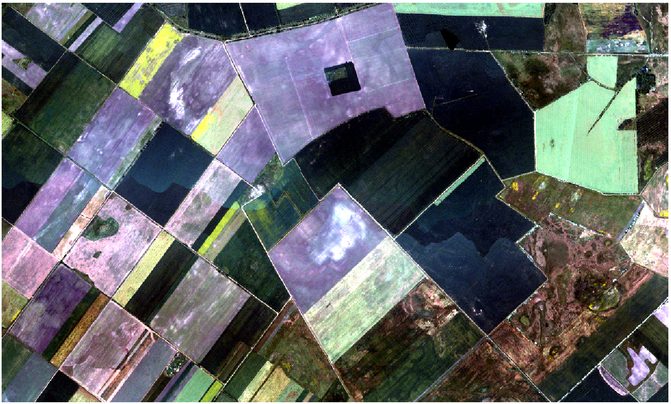
\includegraphics[width=0.7\columnwidth]{Fig/aisa.png} \\
            {\bfseries{(a)}} \\
            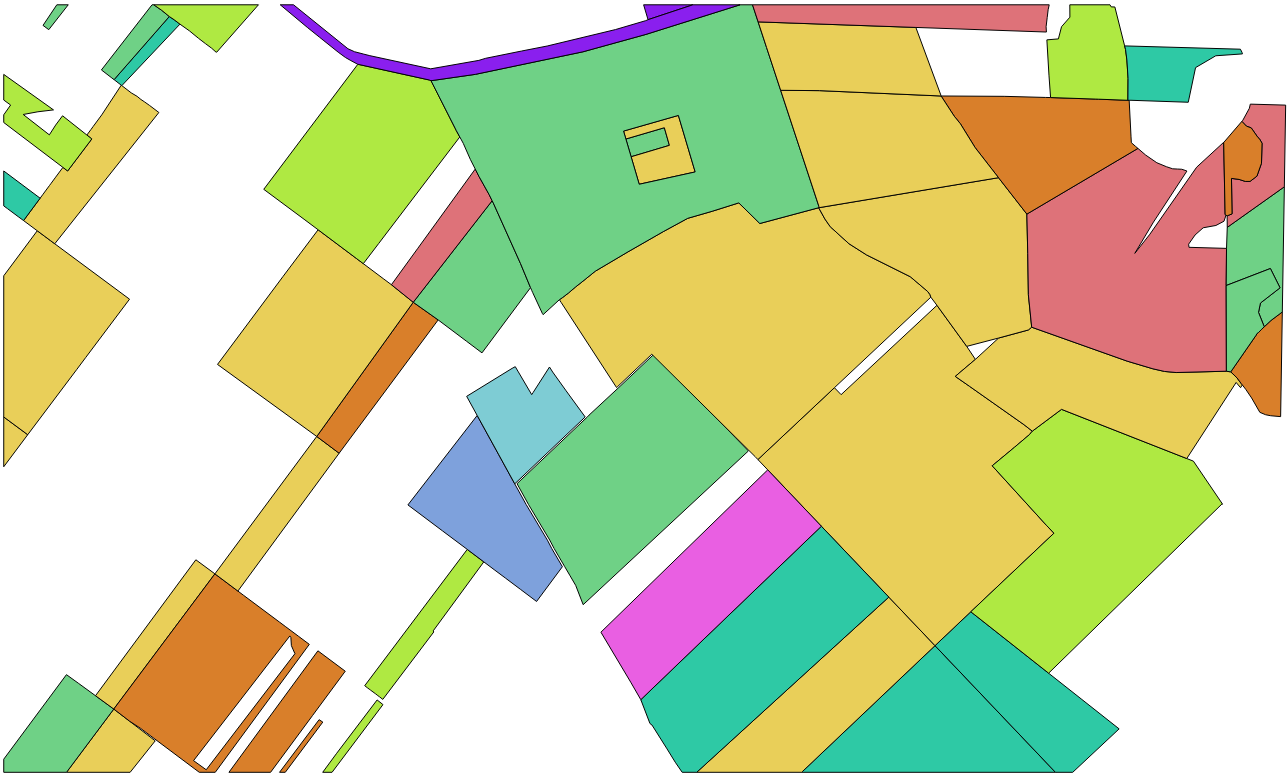
\includegraphics[width=0.7\columnwidth]{Fig/aisa_gt.png} \\
            {\bfseries{(b)}} \\
        \end{tabular}
        \caption{Aisa dataset: {\bfseries{(a)}} colored composition of the image (R: 634nm, G: 519nm, B: 477nm), {\bfseries{(b)}} ground-truth.\label{fig:aisa}}
    \end{figure}

    \begin{table}[!t]
        \centering
        \caption{Information classes for the Aisa dataset.\label{tab:aisa}}
        \begin{tabular}[b]{lc}\toprule
          Class & Number of samples \\ \midrule
          Winter wheat & 136,524 \\
          Sunflower & 61,517 \\
          Green fallow last year treatment & 30,197 \\
          Alfalfa & 17,626 \\
          Maize & 18,278 \\
          Millet & 7,199 \\
          Broadleaved forest & 10,746 \\
          Meadow & 23,283 \\
          Winter barley & 2,799 \\
          Reed & 4,222 \\
          Water course & 4,773 \\
          Rape & 26,566 \\
          Green fallow with shrub & 9,272 \\
          Green fallow last year treated & 3,426 \\
          Pasture & 2,107 \\
          Oat & 3,436 \\ \bottomrule
        \end{tabular}
    \end{table}

    \subsection{Potsdam dataset}
    \label{sec:pots-dataset}

    This  second dataset  is built  from a  dataset of  remote sensing
    images distributed by the International Society for Photogrammetry
    and                         Remote                         Sensing
    (ISPRS)\footnote{\url{http://www2.isprs.org/commissions/comm3/wg4/2d-sem-label-potsdam.html}}. The
    dataset is composed of aerial images of the urban area of Potsdam.
    The area  is divided  into 38  patches of  6000$\times$6000 pixels
    with a  resolution of 5cm by  pixel and 4 channels  are available:
    Red, Blue,  Green and Infrared  (RGBIR).  A Digital  Surface Model
    with  the  same  resolution  is  also  provided  and  a  so-called
    normalized  DSM   representing  the   height  above   ground.  The
    ground-truth  for  24  tiles  are provided  with  6  classes:  Low
    vegetation, High vegetation, Impervious surfaces, Buildings, Cars,
    Clutter.   Three tiles  have  been  used in  this  work, they  are
    displayed             in            Figure~\ref{fig:potsdam-expl}.
    Table~\ref{tab:potsdam} summarizes  the number of samples  of each
    class.

    \begin{figure}[!t]
        \centering
        \begin{tabular}{c@{~}c@{~}c}
            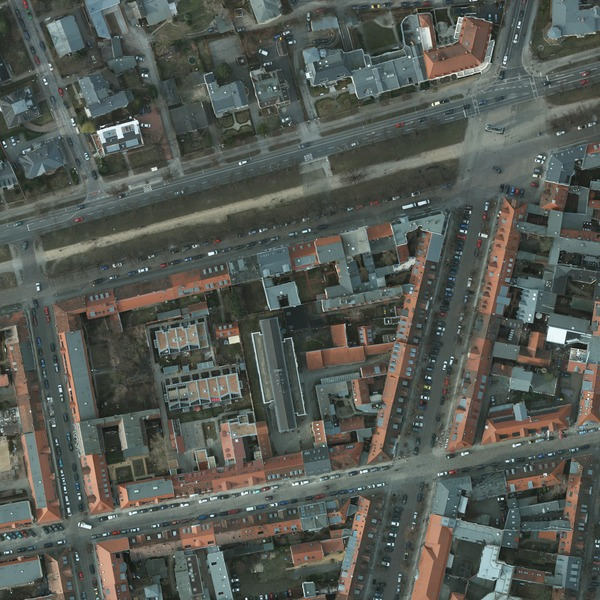
\includegraphics[width=0.3\columnwidth]{Fig/top_potsdam_5_11_RGB.jpg} &
            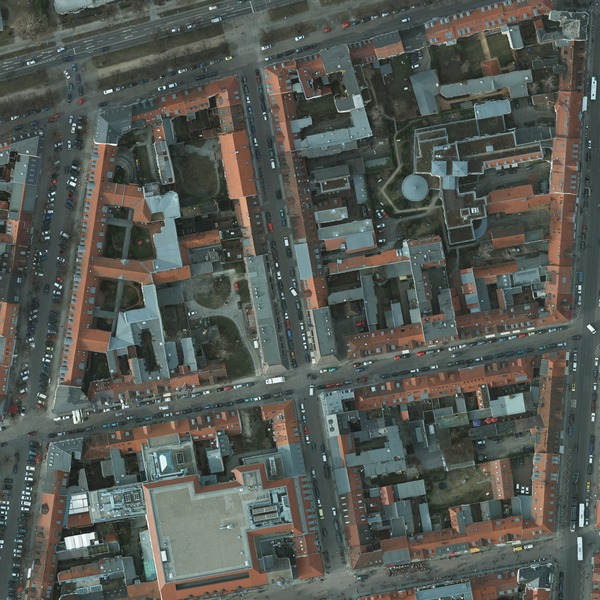
\includegraphics[width=0.3\columnwidth]{Fig/top_potsdam_5_12_RGB.jpg} &
            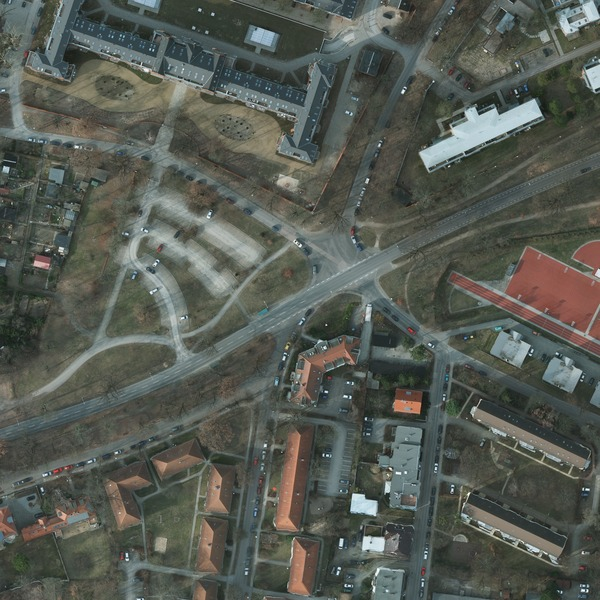
\includegraphics[width=0.3\columnwidth]{Fig/top_potsdam_3_10_RGB.jpg} \\
            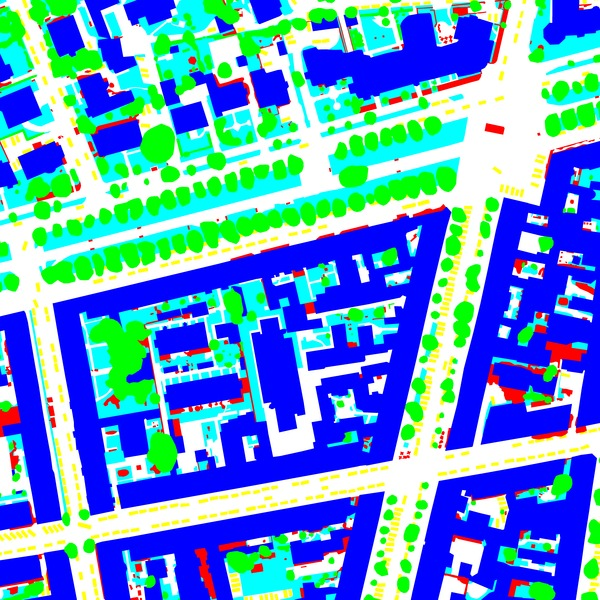
\includegraphics[width=0.3\columnwidth]{Fig/top_potsdam_5_11_label.jpg} &
            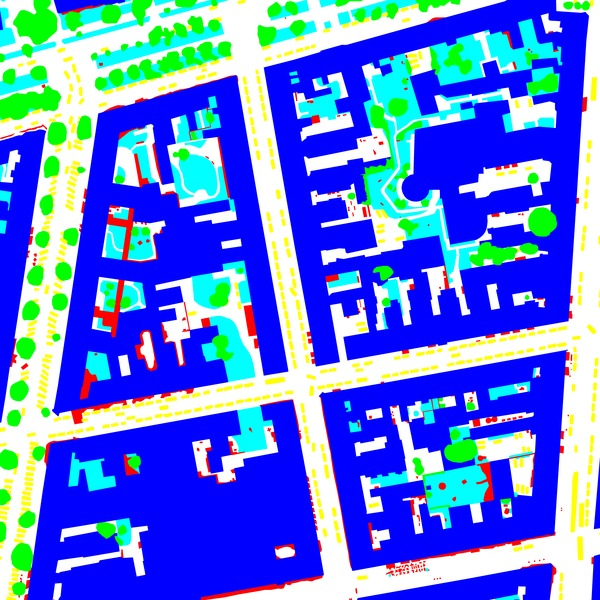
\includegraphics[width=0.3\columnwidth]{Fig/top_potsdam_5_12_label.jpg} &
            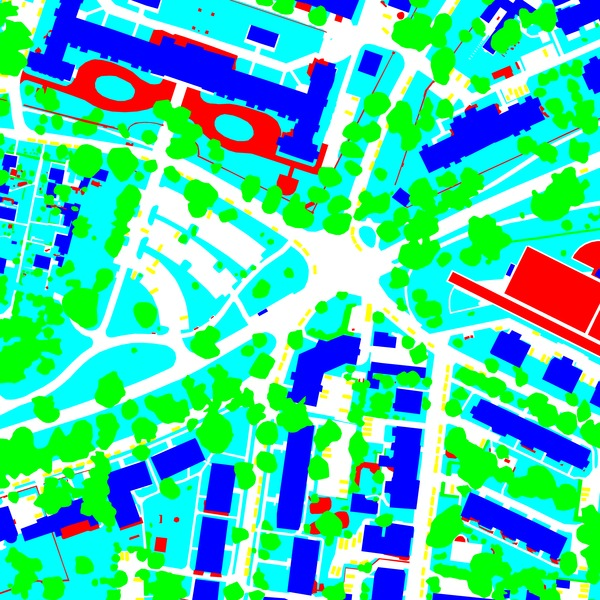
\includegraphics[width=0.3\columnwidth]{Fig/top_potsdam_3_10_label.jpg} \\
            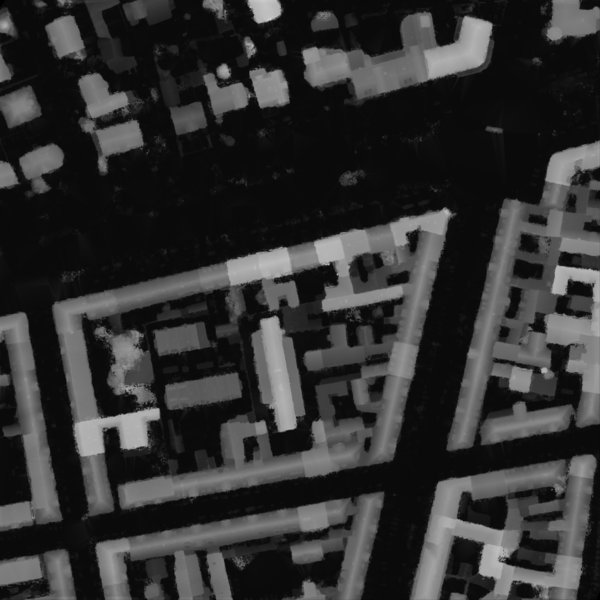
\includegraphics[width=0.3\columnwidth]{Fig/dsm_potsdam_05_11_normalized_lastools.jpg} &
            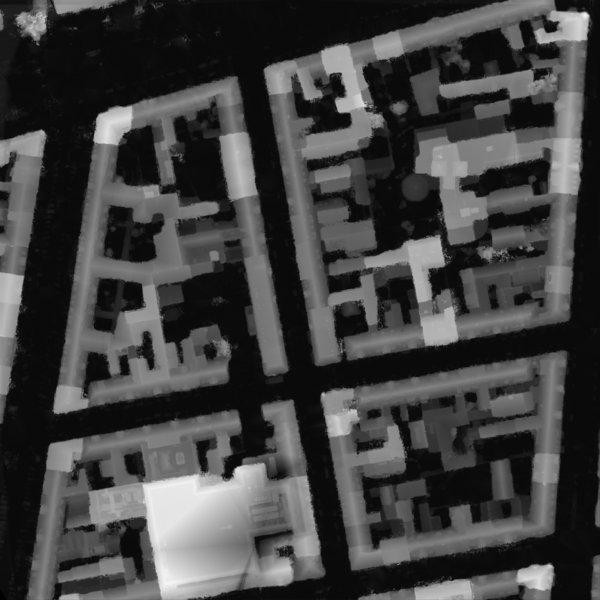
\includegraphics[width=0.3\columnwidth]{Fig/dsm_potsdam_05_12_normalized_lastools.jpg} &
            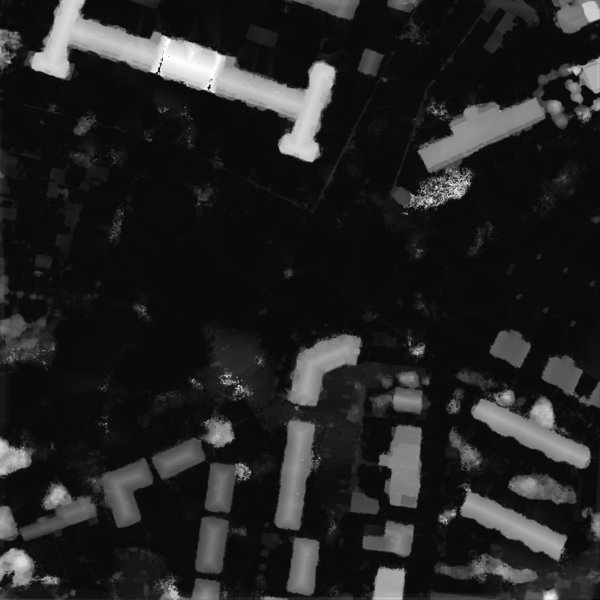
\includegraphics[width=0.3\columnwidth]{Fig/dsm_potsdam_03_10_normalized_lastools.jpg} \\
            {\bfseries{(a)}} & {\bfseries{(b)}}  & {\bfseries{(c)}}\\
        \end{tabular}
        \caption{From top to bottom, true color composition, ground-truth and normalized DSM of: {\bfseries{(a)}} tile 5\_11, {\bfseries{(b)}} tile 5\_12 and {\bfseries{(c)}} tile 3\_10.\label{fig:potsdam-expl}}
    \end{figure}

    \begin{table}[!t]
        \centering
        \caption{Information classes for the three tiles of the Postdam dataset.\label{tab:potsdam}}
        \begin{tabular}[b]{lrrr}\toprule
          & \multicolumn{3}{c}{Number of samples per tile}\\
            \cmidrule{2-4}
            Class &   5\_11  &   5\_12  & 3\_10 \\
          \midrule
          Clutter             & 1,078,611  & 812,038    & 1,890,467 \\
          Trees               & 4,493,295  & 2,132,368  & 8,780,245 \\
          Cars                & 900,076    & 1,101,541  & 434,615 \\
          Buildings           & 13,469,575 & 17,501,421 & 5,128,149 \\
          Low vegetation      & 4,718,219  & 3,210,596  & 11,428,326 \\
          Impervious surfaces & 11,340,224 & 11,242,036 & 8,338,198 \\
          \bottomrule
        \end{tabular}
    \end{table}

    In order to increase the dimensionality of the data, the following features are computed using the RGBIR images similarly to \cite{tuia2015multiclass}:
    \begin{itemize}
        \item Fifteen Radiometric indexes: NDVI, TNDVI, RVI, SAVI, TSAVI, MSAVI, MSAVI2, GEMI, IPVI, NDWI2, NDTI, RI, CI, BI, BI2~\cite{otb}.
        \item Morphological profile build on each band with a disk of radius 5, 9, 13, 17, 21, 25, 29, 33, 37 and 41 (80 features)~\cite{fauvel2013advances};
        \item Attribute profile build on each band with area as attribute and 1000, 2000, 5000, 10000 and 15000 as thresholds (40 features)~\cite{dalla2010morphological}.
        \item Attribute profile build on each band with diagonal of bounding box as attribute and 100, 200, 500, 1000 and 20000 as thresholds (40 features)~\cite{dalla2010morphological}.
        \item Textural features for  each channel with neighborhood of
          19x19 pixels:  mean, standard  deviation, range  and entropy
          (16 features)~\cite{otb}.
    \end{itemize}
    The normalized DSM and the raw  RGBIR image are added to these 191
    features and  then stacked to  create a  new image  with 196
    bands. %  The  training is  made with  tile 5\_11  and test  with two
    % tiles: 5\_12 which very similar with  tile 5\_11 and 3\_10 which a
    % further area a bit less urban and more industrial.


\section{Experimental results}
\label{sec:test}

    \subsection{Method}
    \label{sec:method}

    The aim  of the experiments is  to compare the proposed  method to
    standard    classifiers    used    in   operational    land    map
    production~\cite{rs70912356}. A non-optimized  previous version of
    the method has been already compared to other selection methods in
    \cite{fauvel2015fast}.  Hence, the primary  objective is to assess
    the  operational  efficiency  and  it is  compared  to  other  OTB
    classifiers   used  operationally   through  their   command  line
    applications\footnote{\url{http://otbcb.readthedocs.io/en/latest/OTB-Applications.html}}.

    The following classifiers are tested:
    \begin{itemize}
        \item A k-nearest-neighbors classifier (KNN) with OTB default parameters (32 as number of neighbors).
        \item A Random Forest classifier with parameters optimized by grid search (200 trees, 40 as max depth, 50 as size of the randomly selected subset of features at each tree node)
        \item A GMM classifier with ridge regularization (GMM ridge) with regularization constant optimized by grid search.
    \end{itemize}
    The GMM classifier is part of the external module described in Section~\ref{sec:otb-module}.

    All these classifiers are compared with 3 configurations of the proposed GMM classifier:
    \begin{itemize}
    \item One with forward selection and JM distance as criterion (GMM SFS JM);
    \item One with forward selection and Cohen's kappa as criterion (GMM SFS kappa);
    \item One with floating forward selection and JM distance as criterion (GMM SFFS JM).
    \end{itemize}
    Other configurations  have been  investigated and  performs either
    equally     or     lower     in    terms     of     classification
    accuracy~\cite{al:report}. For the sake of clarity, only the three
    aforementioned configurations are discussed here.

    The training set has been created  with an equal number of samples
    for each class and additionally  a spatial stratification has been
    performed, \emph{i.e.}, each training  sample belongs to a spatial
    polygon  that  does  not  intersect  spatially  with  any  spatial
    polygons used  for the validation.   Several size of  training set
    have been  tested.  For  the Aisa  dataset, experiments  have been
    conducted using  250, 500 and  1000 samples  by class and  for the
    Potsdam dataset, 1000 and 50000 samples by class.

    For SFS and  SFFS selection, the number of variables  to select is
    set to  30 for the  Aisa dataset and  60 for the  Potsdam dataset.
    After  the selection  procedure, the  optimal number  of extracted
    variables is selected as follow.  Rather than selecting the number
    of variables corresponding to the  highest value of the criterion,
    the number of  retained variables is set when  the criterion stops
    to increase significantly.  It is  found by computing the discrete
    derivative of the criteria.  See Figure~\ref{fig:crit-evol} for an
    example.

    \begin{figure}[!t]
        \centering
        \begin{tikzpicture}
            \begin{axis}[ymin=0.2,ymax=0.9,grid,axis x line=left,axis y line=left,xlabel={\# variables},ylabel={Cohen's kappa},small]
                \addplot[thick,black] table[x=nb,y=crit] {criterion_1000spl_aisa.txt};
                \draw[thick,red] (axis cs:18,\pgfkeysvalueof{/pgfplots/ymin}) -- (axis cs:18,\pgfkeysvalueof{/pgfplots/ymax});
                \draw[thick,black] (axis cs:24,\pgfkeysvalueof{/pgfplots/ymin}) -- (axis cs:24,\pgfkeysvalueof{/pgfplots/ymax});
            \end{axis};
            % \begin{axis}[ymin=0.2,ymax=0.75,grid,axis x line=left,axis y line=left,xlabel={\# variables},ylabel={Cohen's kappa},small]
            %     \addplot[thick,black] table[x=nb,y=crit] {criterion_1000spl.txt};
            %     \draw[thick,red] (axis cs:15,\pgfkeysvalueof{/pgfplots/ymin}) -- (axis cs:15,\pgfkeysvalueof{/pgfplots/ymax});
            %     \draw[thick,black] (axis cs:47,\pgfkeysvalueof{/pgfplots/ymin}) -- (axis cs:47,\pgfkeysvalueof{/pgfplots/ymax});
            % \end{axis};
            % \begin{axis}[ymin=0.2,ymax=0.75,grid,axis x line=left,axis y line=left,xlabel={\# variables},ylabel={Cohen's kappa}]
            %     \addplot[thick,black] table[x=nb,y=crit] {criterion_50000spl.txt};
            %     \draw[thick,red] (axis cs:31,\pgfkeysvalueof{/pgfplots/ymin}) -- (axis cs:31,\pgfkeysvalueof{/pgfplots/ymax});
            %     \draw[thick,black] (axis cs:31,\pgfkeysvalueof{/pgfplots/ymin}) -- (axis cs:31,\pgfkeysvalueof{/pgfplots/ymax});
            % \end{axis};
        \end{tikzpicture}
        \caption{Criterion evolution (kappa) in function of the number of selected variables for first trial with Aisa dataset with 500 samples by class. Red vertical line is the retained number of variables and black vertical line is the maximum of the criterion.\label{fig:crit-evol}}
    \end{figure}

    % Then, a small processing is made to select the number of variables used for prediction. The evolution of the criterion function is retrieved from the model file and the discrete derivative of the criterion \emph{DJ} is computed and normalized by its maximum. The subset of variables used for classification $\Omega^{*}$ is the first subset for which this value is lower than a given threshold \emph{th}, equal  to 0.1\% in this experiment,
    % \begin{equation*}
    %     \Omega^{*} = \Omega_{\min \{k|DJ_k<th\}}
    % \end{equation*}
    % with $DJ_k = \frac{J(\Omega_k) - J(\Omega_{k-1})}{\max_k (J(\Omega_k) - J(\Omega_{k-1}))}$.

    The    classification   rate    is    presented   using    Cohen's
    kappa. Processing  time has been  evaluated on a  desktop computer
    with  8Gb of  RAM  and  Intel(R) Core(TM)  i5-3570  CPU @  3.40GHz
    $\times$ 4 processors.

    \subsection{Aisa dataset}
    \label{sec:aisa}

    When creating training and validation  sets, special care is taken
    to assure that training samples are picked out from distinct areas
    than test  samples.  The  polygons of the  reference are  split in
    smaller polygons and then 50\%  of the polygons are taken randomly
    for training and the remaining 50\% for validation.  An example of
    training      and     validation      set     is      shown     in
    Figure~\ref{fig:set-aisa}.  From the  training  polygons, a  given
    number of samples  were selected to build the  training set, while
    all  the pixels  from the  validation polygons  were used  for the
    validation.  Moreover 20  random trials were run  with a different
    training  set (different  polygons).  Table~\ref{tab:aisa-otbsimu}
    presents  the results  of the  experiment with  mean and  standard
    deviation  of  the  Kappa  coefficient  over  the  20  trials  and
    Table~\ref{tab:aisa-otbsimu-time}  the   corresponding  processing
    time. Bold values corresponds to best results. In Table~\ref{tab:aisa-otbsimu}, when several bold scores appears for the same experiment, it means that the scores has been assessed as equivalent with a Wilcoxon rank-sum test \cite{mann1947test}. Additionally, Figure~\ref{fig:meanNbVar-aisa} summarizes the mean of the number of selected variables for each variation of the GMM classifier with selection.

    \begin{figure}[!t]
        \centering
        \begin{tabular}{c}
            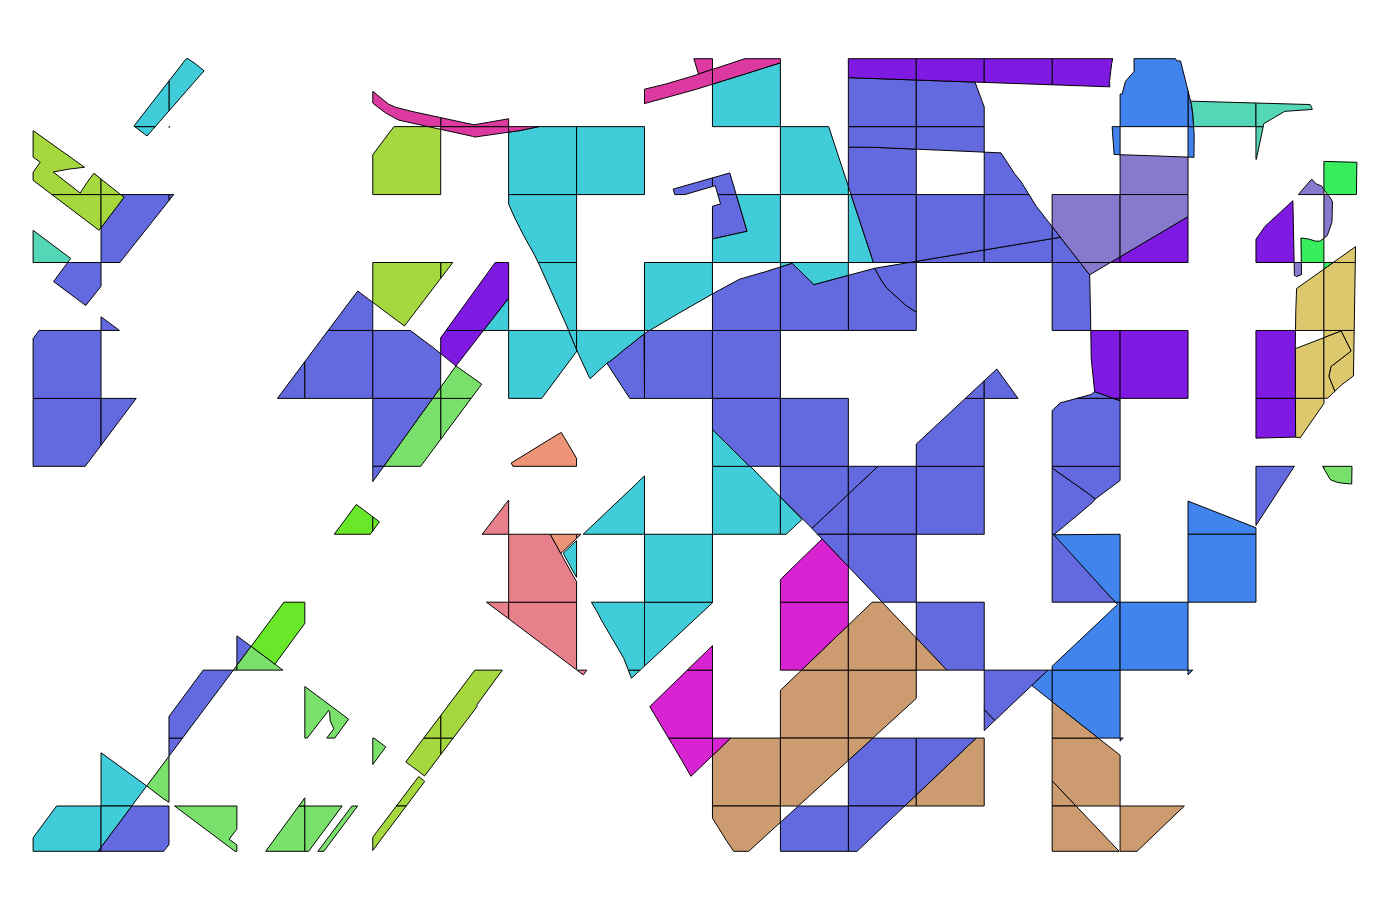
\includegraphics[width=0.7\columnwidth]{Fig/aisa_gt_train.png} \\
            {\bfseries{(a)}} \\
            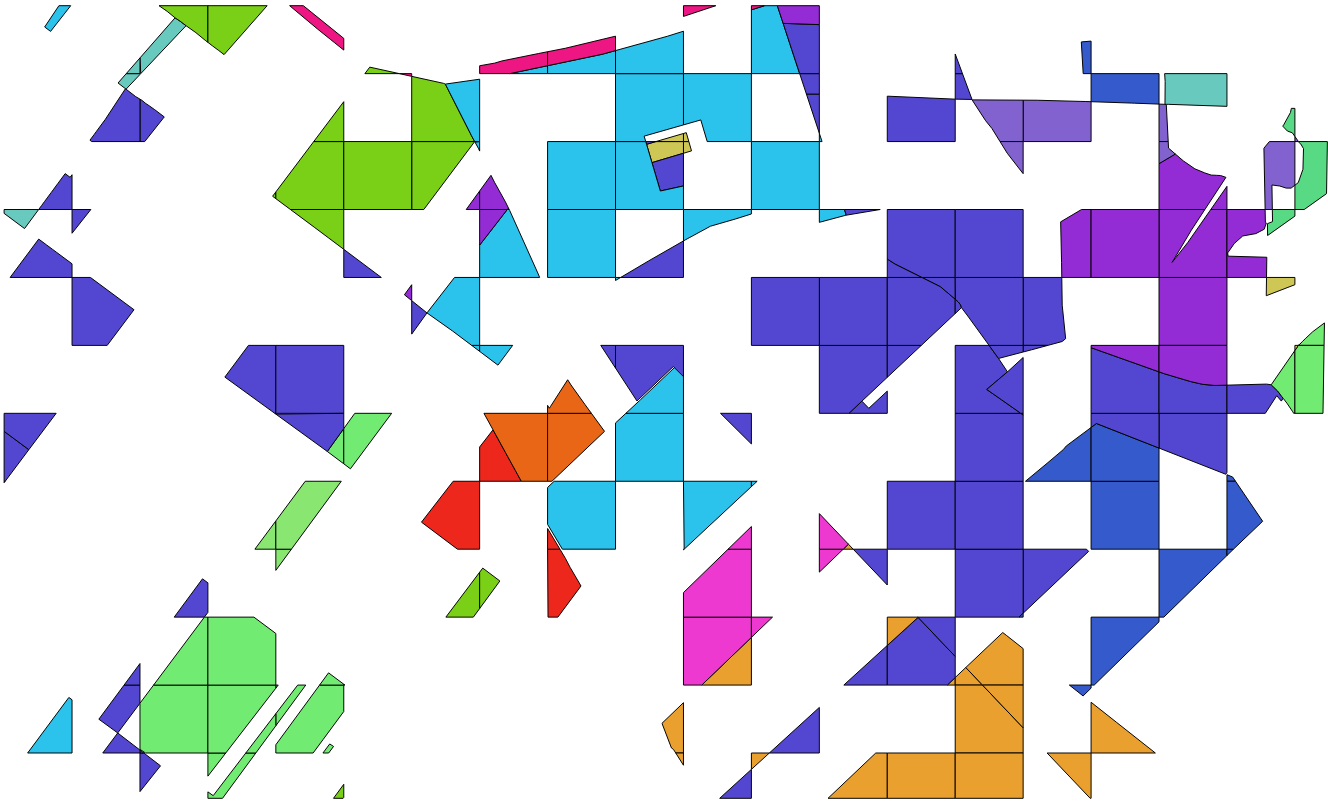
\includegraphics[width=0.7\columnwidth]{Fig/aisa_gt_test.png} \\
            {\bfseries{(b)}} \\
        \end{tabular}
        \caption{Aisa dataset: {\bfseries{(a)}} training polygons of first trial, {\bfseries{(b)}} test polygons of first trial.\label{fig:set-aisa}}
    \end{figure}

    \begin{table}[!t]
        \centering
        \caption{Average classification accuracy 20 trials (standard deviation in parenthesis).\label{tab:aisa-otbsimu}}
        \begin{tabular}{lccc}\toprule
             & \multicolumn{3}{c}{\bfseries Cohen's kappa} \\ \cmidrule{2-4}
            \# samples by class & 250 & 500 & 1000 \\ \midrule

            GMM SFS kappa & {\bfseries 0.678 (0.029)} & {\bfseries 0.687 (0.029)} & {\bfseries 0.699 (0.028)} \\
            GMM SFS JM &    {\bfseries 0.685 (0.030)} & {\bfseries 0.689 (0.030)} & {\bfseries 0.701 (0.029)} \\
            GMM SFFS JM &   {\bfseries 0.685 (0.030)} & {\bfseries 0.689 (0.030)} & {\bfseries 0.701 (0.029)} \\
            GMM ridge &     0.611 (0.040) & 0.620 (0.036) & 0.642 (0.034) \\
            KNN &           0.551 (0.035) & 0.563 (0.033) & 0.574 (0.030) \\
            Random Forest & 0.645 (0.026) & 0.673 (0.023) & {\bfseries 0.693 (0.023)} \\
            \bottomrule
        \end{tabular}
    \end{table}

    % this one is result without changing the number of selected variables
    % \begin{table}[!t]
    %     \centering
    %     \caption{Average classification accuracy 20 trials (standard deviation in parenthesis).\label{tab:aisa-otbsimu}}
    %     \begin{tabular}{lccc}\toprule
    %          & \multicolumn{3}{c}{\bfseries Cohen's kappa} \\ \cmidrule{2-4}
    %         \# samples by class & 250 & 500 & 1000 \\ \midrule

    %         GMM SFS kappa & {\bfseries 0.684 (0.025)} & {\bfseries 0.698 (0.027)} & {\bfseries 0.711 (0.028)} \\
    %         GMM SFS JM &    {\bfseries 0.680 (0.028)} & {\bfseries 0.700 (0.028)} & {\bfseries 0.710 (0.030)} \\
    %         GMM SFFS JM &   {\bfseries 0.680 (0.028)} & {\bfseries 0.700 (0.028)} & {\bfseries 0.710 (0.030)} \\
    %         GMM ridge &     0.611 (0.040) & 0.620 (0.036) & 0.642 (0.034) \\
    %         KNN &           0.551 (0.035) & 0.563 (0.033) & 0.574 (0.030) \\
    %         Random Forest & 0.645 (0.026) & 0.673 (0.023) & 0.693 (0.023) \\
    %         \bottomrule
    %     \end{tabular}
    % \end{table}

    \begin{figure}
      \centering
      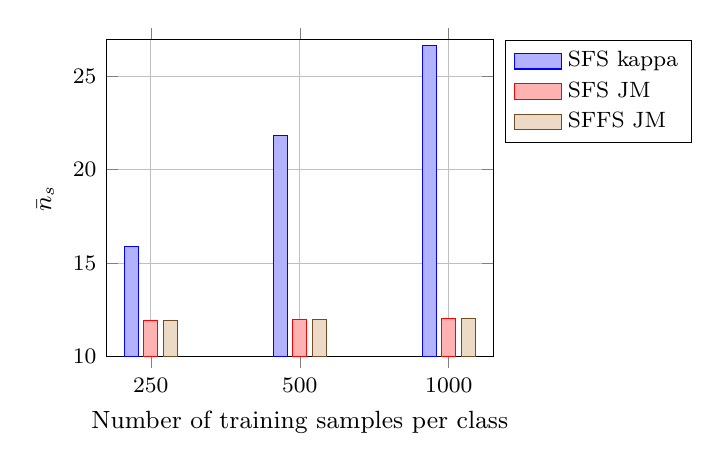
\begin{tikzpicture}
        \begin{axis}[ylabel=$\bar{n}_s$,ymax=25,
          symbolic x coords={0,250,500,1000,1050},
          enlargelimits=0.15,legend pos=outer north east,xtick=data,legend cell align=left,
          ybar,
          bar width=5pt,grid,xlabel=Number of training samples per class,small,area legend]
          \addplot coordinates {(250,15.9) (500,21.85) (1000,26.65)};
          \addplot coordinates {(250,11.95) (500,12) (1000,12.05)};
          \addplot coordinates {(250,11.95) (500,12) (1000,12.05)};
          %%\addplot[red,very thick,sharp plot,update limits=false]coordinates {(0,252) (1050,252)};
          \legend{{\footnotesize SFS kappa},{\footnotesize SFS JM},{\footnotesize SFFS JM}}
        \end{axis}
      \end{tikzpicture}
      \caption{Mean number $\bar{n}_s$ of selected features for the different variation of selection methods for Aisa data set. The original number of features is 252.}
      \label{fig:meanNbVar-aisa}
    \end{figure}

    \begin{table}[!t]
        \centering
        \caption{Mean processing time for training and classification for results in Table \ref{tab:aisa-otbsimu}.\label{tab:aisa-otbsimu-time}}
        \begin{tabularx}{\columnwidth}{l*{6}{>{\centering\arraybackslash}X}}
            \toprule
             & \multicolumn{3}{c}{\bfseries Training time (s)} & \multicolumn{3}{c}{\bfseries Classification time (s)} \\ \cmidrule{2-7}
            \# samples by class & 250 & 500 & 1000 & 250 & 500 & 1000 \\ \midrule

            GMM SFS kappa & 257             & 496             & 955             & {\bfseries 5.2} & {\bfseries 5.2} & {\bfseries 5.5} \\
            GMM SFS JM &    {\bfseries 8.6} & {\bfseries 8.9} & {\bfseries 9.1} & {\bfseries 5.7} & {\bfseries 5.7} & {\bfseries 5.9} \\
            GMM SFFS JM &   {\bfseries 8.8} & {\bfseries 9.0} & {\bfseries 9.3} & {\bfseries 5.0} & {\bfseries 5.0} & {\bfseries 5.4} \\
            GMM ridge &     71.7            & 105             & 167             & 530 & 530 & 530 \\
            KNN &           {\bfseries 8.9} & 19.6            & 59.7            & 387 & 639 & 887 \\
            Random Forest & 24.5            & 49.3            & 105             & 33.0 & 41.7 & 45.9 \\
            \bottomrule
        \end{tabularx}
    \end{table}

    The results show that, on this  dataset, GMM classifiers with feature selection get the best classification rate. Among the three variations of the selection algorithm, none appears to perform better than the others. Using kappa or Jeffries-Matusita distance as criterion is equal and using SFFS does not give any advantage.

    The difference with the second best classifier, Random Forest, appears to be significant when using 250 and 500 samples. Random Forest has similar performance in term of classification rate with 1000 samples. The GMM classifier with ridge regularization and the KNN classifier are both outperformed.

    In term of computational time, the GMM classifiers are as expected very fast for classification and also for training, except when the criterion function is a classification rate. In this case, using JM distance as criterion and SFS as search strategy is the best choice in term of time efficiency. The good performance in time can be explained by the dimension reduction. Actually, the decision rule corresponding to Equation~(\ref{eq:decision}) has a complexity in $d^3$ where $d$ is the dimension. Thus, reducing $d$ induces a reduction of the classification time.

    The processing times of the three standard classifiers suffer from the increase of training samples. For the GMM classifier with ridge, the selection of regularization parameter is more costly with more samples because of the classification rate estimation needed. For the KNN classifier, the model stores all the training samples and the prediction implies to compute the distance to all the training samples which explains the increase of the processing time and additionally of the size of the model file. Finally, for the Random Forest classifier, the trees tends to be deeper in order to capture the additional information available with more samples and that explains the increase of the processing time.
    % The computation of the kappa seems  to suffer from  a lack of  parallelization   which could be  improved. ->  plus tard dans la conclusion.

    \subsection{Potsdam dataset}

    For the Potsdam  dataset, training samples were  selected from one
    tile (5\_11)  and validation  samples were all  the pixel  of tile
    5\_12     or    3\_10.      Table~\ref{tab:potsdam-otbsimu}    and
    Table~\ref{tab:potsdam-otbsimu-big} present  the results  in terms
    of classification accuracy and processing time. Bold values corresponds to best results. In Table~\ref{tab:potsdam-otbsimu}, when several bold scores appears for the same experiment, it means that the scores has been assessed as equivalent with a Wilcoxon rank-sum test \cite{mann1947test}.

    \begin{table*}[!t]
        \centering
        \caption{Kappa coefficient and processing time for 1,000 samples by class and averaged over 5 trials (standard deviation in parenthesis). Processing times are given in second.\label{tab:potsdam-otbsimu}}
        \begin{tabular}{lcccccc}\toprule
            & {\bfseries 5\_11 (train)} & {\bfseries 5\_12 (test)} & {\bfseries 3\_10 (test)} & {\bfseries Train. Time} & {\bfseries Classif. time} & {\bfseries \# of selected features} \\ \cmidrule{2-7}
            GMM SFS kappa & 0.694 (0.002)             & {\bfseries 0.669 (0.005)} & {\bfseries 0.533 (0.008)} & 400 & 310  & 13.2 \\
            GMM SFS JM &    0.624 (0.028)             & 0.631 (0.034)             & 0.461 (0.027)             & 2   & 310  & 11 \\
            GMM SFFS JM &   0.624 (0.028)             & 0.631 (0.034)             & 0.461 (0.027)             & 2.6 & 310  & 11 \\
            GMM ridge &     0.632 (0.007)             & 0.592 (0.010)             & 0.433 (0.008)             & 10  & 2000 & all \\
            KNN &           0.637 (0.005)             & 0.607 (0.005)             & 0.478 (0.002)             & 0.7 & 9500 & all \\
            Random Forest & {\bfseries 0.729 (0.004)} & {\bfseries 0.673 (0.005)} & {\bfseries 0.529 (0.009)} & 20  & 840  & all \\
            \bottomrule
        \end{tabular}
    \end{table*}

    \begin{table*}[!t]
        \centering
        \caption{Kappa coefficient and processing time for 50,000 samples by class and averaged over 5 trials (standard deviation in parenthesis). Processing times are given in second. NB: the test has not been conduct with KNN because of a too long processing time for classification.\label{tab:potsdam-otbsimu-big}}
        \begin{tabular}{lcccccc}\toprule
            & {\bfseries 5\_11 (train)} & {\bfseries 5\_12 (test)} & {\bfseries 3\_10 (test)} & {\bfseries Train. Time} & {\bfseries Classif. time} & {\bfseries \# of selected features} \\ \cmidrule{2-7}
            GMM SFS kappa & 0.713 (0.001) & 0.684 (0.001) & 0.531 (0.005) & 20000 & 340 & 29 \\
            GMM SFS JM &    0.560 (0.111) & 0.576 (0.104) & 0.435 (0.085) & 6 & 330 & 10 \\
            GMM SFFS JM &   0.560 (0.111) & 0.576 (0.104) & 0.435 (0.085) & 6.6 & 340 & 10 \\
            GMM ridge &     0.641 (0.015) & 0.611 (0.026) & 0.440 (0.015) & 460 & 2000 & all \\
            KNN &           /             & /             & /             & / & / & / \\
            Random Forest & {\bfseries 0.851 (0.001)} & {\bfseries 0.715 (0.001)} & {\bfseries 0.573 (0.002)} & 2000 & 2000 & all \\
            \bottomrule
        \end{tabular}
    \end{table*}

    With this second dataset, the Random Forest classifier and the GMM classifier with kappa as selection criterion perform the best in terms of classification accuracy. When using 1000 samples per class, no significant difference of classification rate has been observed on test set. But, with 50,000 samples per class, the Random Forest classifier becomes significantly better in terms of classification accuracy.

    % It can be guessed that the fact that the Gaussian hypothesis is unlikely to be verified explains the difficulty to extract the finer information available in a larger dataset. The JM distance has stressed in Table~\ref{tab:crit} has a strong Gaussian hypothesis and the same hypotheses could also explain the drop of the classification rate of GMM classifiers with JM distance as criterion.

    The  Postdam classes  are  more difficult  to discriminate,  since
    Gaussianity assumption  does not  hold. For instance,  a buildings
    can  be  made of  various  materials,  resulting in  heterogeneous
    distribution.   Hence,  GMM  with  ridge  regularization  performs
    baldy. Random  Forest classifier is  more adapted to  this problem
    and reached the  best classification accuracy. However,  it can be
    note  that letting  the algorithm  be driven  by a  classification
    quality criterion such as the Kappa coefficient helps in improving
    the  classification   accuracy.  The   KNN  classifier   is  again
    outperformed.

    From        the        tables~\ref{tab:potsdam-otbsimu}        and
    Table~\ref{tab:potsdam-otbsimu-big},   the  number   of  extracted
    variables shows that JM criterion identifies less relevant samples
    than with the kappa criterion. Moreover, the selection method with
    criterion kappa manages to get good performance with only 6.7\% of
    the  initial variables  with  1000 samples  and  15\% with  50,000
    samples.

    In term of processing time, results are similar than with the Aisa
    dataset.  GMM  classifiers  with   selection  are  very  fast  for
    prediction.  For  example,  the   GMM  classifier  with  kappa  as
    criterion for the selection is  63\% faster than the Random Forest
    classifier for prediction  with 1000 samples and  83\% faster with
    50,000  samples.  However, the  training  time  is increased  with
    respect to random forest.

\section{Conclusion and perspectives}
\label{sec:conclusion}

An algorithm for the classification of high dimensional Earth observation images has been proposed. The algorithm is based on Gaussian mixture model and a forward feature selection strategy to reduce the dimension of the data to be processed. From experimental results, this strategy has shown to be robust the \emph{curse of dimensionality}. As a side effect, the volume of data is reduced and the final classification processing time is reduced. 

To cope with the large volume of data during the learning step, updates rules from the forward search have been split into two parts in order to save computation. One part is only computed once per iteration, and the other part needs to be computed for each tested features. Several criteria have been included, three based on classification accuracy and two based on divergence measures.

Experiments have been conducted on two real high dimensional data set, and the results have been compared to standards classifiers. Results show that the proposed approach  performs, in most cases, at least as best as classifiers (Random Forest) and even outperforms all of them in term of classification time.

The resulting code is available as a remote module of the Orfeo toolbox on Github and makes it possible to process large high dimensional images efficiently. The \texttt{C++} code is freely available for download: \url{https://www.orfeo-toolbox.org/external-projects/}.

Perspectives of this work concern the selection of continuous interval of features rather than a single feature~\cite{serpico2007extraction,1468090}. It will be of  highest interest for continuous features, such as temporal feature or spectral feature.

% Finally, an improvement could be made to increase the stability of the selected features. For example, with hyperspectral data, a selection of continuous intervals and not band is a possible solution which has already been explored in \cite{serpico2007extraction}.

% The python and C++ code are available freely for download: \url{https://www.orfeo-toolbox.org/external-projects/}, .

\appendices
\section{Proof of update rules}
\label{app:proof-update}
    % \subsubsection{Proposition~(\ref{eq:update-inv-back})}
    %     \begin{proof}
    %         \begin{align*}
    %             \mathbf{A} - \alpha \mathbf{v} \mathbf{v}^t
    %             &= (\boldsymbol{\Sigma}^{(k-1)})^{-1} + \frac{1}{\alpha} (\boldsymbol{\Sigma}^{(k-1)})^{-1} \mathbf{u} \mathbf{u}^t (\boldsymbol{\Sigma}^{(k-1)})^{-1} \\
    %             &~~~- \alpha (- \frac{1}{\alpha} (\boldsymbol{\Sigma}^{(k-1)})^{-1} \mathbf{u}) (- \frac{1}{\alpha} \mathbf{u}^t (\boldsymbol{\Sigma}^{(k-1)})^{-1})) \\
    %             &= (\boldsymbol{\Sigma}^{(k-1)})^{-1}
    %         \end{align*}
    %     \end{proof}

\begin{proof}[Proof of proposition~(\ref{eq:update-quad})]
    \begin{alignat*}{3}
    (&\mathbf{x}^{(k)})^t && (\boldsymbol{\Sigma}^{(k)}_c)^{-1} \mathbf{x}^{(k)} \\
     &= &&\left[\begin{array}{cc} (\mathbf{x}^{(k-1)})^t   & x_k \end{array}\right]
        \left[\begin{array}{cc}
            \mathbf{A}_c   & \mathbf{v}_c \\
            \mathbf{v}_c^t & \frac{1}{\alpha_c}
        \end{array}\right]
        \left[\begin{array}{c} \mathbf{x}^{(k-1)} \\ x_k \end{array}\right] \\
     &= &&\left[\begin{array}{cc} (\mathbf{x}^{(k-1)})^t   & x_k \end{array}\right]
            \left[\begin{array}{c} \mathbf{A}_c \mathbf{x}^{(k-1)} + x_k \mathbf{v}_c \\ \mathbf{v}_c^t \mathbf{x}^{(k-1)} + \frac{x_k}{\alpha_c} \end{array}\right] \\
     &= &&(\mathbf{x}^{(k-1)})^t \mathbf{A}_c \mathbf{x}^{(k-1)} + x_k \mathbf{v}_c^t \mathbf{x}^{(k-1)} \\
     & &&+ (\mathbf{x}^{(k-1)})^t \mathbf{v}_c x_k + \frac{(x_k)^2}{\alpha_c} \\
     &= &&(\mathbf{x}^{(k-1)})^t \Big((\boldsymbol{\Sigma}_c^{(k-1)})^{-1} \\
     & &&+ \frac{1}{\alpha_c} (\boldsymbol{\Sigma}_c^{(k-1)})^{-1} \mathbf{u}_c \mathbf{u}_c^t (\boldsymbol{\Sigma}_c^{(k-1)})^{-1}\Big) \mathbf{x}^{(k-1)}\\
     & &&+ 2 x_k \mathbf{v}_c^t \mathbf{x}^{(k-1)} + \frac{(x_k)^2}{\alpha_c} \\
     &= &&(\mathbf{x}^{(k-1)})^t \Big((\boldsymbol{\Sigma}_c^{(k-1)})^{-1} + \alpha_c \mathbf{v}_c \mathbf{v}_c^t\Big) \mathbf{x}^{(k-1)}\\
     & &&+ 2 x_k \mathbf{v}_c^t \mathbf{x}^{(k-1)} + \frac{(x_k)^2}{\alpha_c} \\
     &= &&(\mathbf{x}^{(k-1)})^t (\boldsymbol{\Sigma}_c^{(k-1)})^{-1} \mathbf{x}^{(k-1)} + \alpha_c \Big( (\mathbf{x}^{(k-1)})^t \mathbf{v}_c \mathbf{v}_c^t \mathbf{x}^{(k-1)} \\
     & &&+ 2 \frac{x_k}{\alpha_c} \mathbf{v}_c^t \mathbf{x}^{(k-1)} + \frac{(x_k)^2}{\alpha_c^2}\Big) \\
     &= &&(\mathbf{x}^{(k-1)})^t (\boldsymbol{\Sigma}_c^{(k-1)})^{-1} \mathbf{x}^{(k-1)} + \alpha_c \Big( (\mathbf{x}^{(k-1)})^t \mathbf{v}_c + \frac{x_k}{\alpha_c} \Big)^2 \\
     &= &&(\mathbf{x}^{(k-1)})^t (\boldsymbol{\Sigma}_c^{(k-1)})^{-1} \mathbf{x}^{(k-1)} + \alpha_c ( \left[\begin{array}{cc} \mathbf{v}_c^t & \frac{1}{\alpha_c} \end{array}\right] \mathbf{x}^{(k)} )^2
    \end{alignat*}
\end{proof}

\begin{proof}[Proof of proposition~(\ref{eq:update-log})]

    % \begin{align*}
    %     \log &\left(|\boldsymbol{\Sigma}_c^{(k)}|\right) =
    %     \log \left(\left|
    %         \bigg[\begin{array}{cc}
    %             \boldsymbol{\Sigma}_c^{(k-1)} & \mathbf{u}_c      \\
    %             \mathbf{u}_c^t          & \sigma^{(k)}_c \\
    %         \end{array}\bigg]
    %     \right|\right) \\
    %     =&\log \left(\left|
    %         \bigg[\begin{array}{cc}
    %             \boldsymbol{\Sigma}_c^{(k-1)} & \mathbf{0}_{k-1,1}     \\
    %             \mathbf{u}_c^t          & 1 \\
    %         \end{array}\bigg]
    %         \bigg[\begin{array}{cc}
    %             \mathbf{I}_{k-1} & (\boldsymbol{\Sigma}_c^{(k-1)})^{-1} \mathbf{u}_c      \\
    %             \mathbf{0}_{k-1,1}^t          & \sigma^{(k)}_c - \mathbf{u}_c^t(\boldsymbol{\Sigma}_c^{(k-1)})^{-1} \mathbf{u}_c\\
    %         \end{array}\bigg]
    %     \right|\right) \\
    %     =&\log \left(\left|
    %         \bigg[\begin{array}{cc}
    %             \boldsymbol{\Sigma}_c^{(k-1)} & \mathbf{0}_{k-1,1}     \\
    %             \mathbf{u}_c^t          & 1 \\
    %         \end{array}\bigg]
    %     \right|\right)
    %     +\log \left(\left|
    %         \bigg[\begin{array}{cc}
    %             \mathbf{I}_{k-1} & (\boldsymbol{\Sigma}_c^{(k-1)})^{-1} \mathbf{u}_c      \\
    %             \mathbf{0}_{k-1,1}^t          & \alpha_c \\
    %         \end{array}\bigg]
    %     \right|\right) \\
    %     =&\log \left( |\boldsymbol{\Sigma}_c^{(k-1)}| |1| \right) + \log \left( |\mathbf{I}_{k-1}| |\alpha_c| \right)\\
    %     =&\log \left( |\boldsymbol{\Sigma}_c^{(k-1)}| \right) + \log ( \alpha_c )
    % \end{align*}
    % \noindent where $\mathbf{I}_{k-1}$ is the $(k-1) \times (k-1)$ identity matrix and $\mathbf{0}_{k-1,1}$ is the $(k-1) \times 1$ null vector.
  From eq.~(\ref{eq:cov}) and standard results for the determinant of block matrix~\cite[Chapter 9]{IMM2012-03274} we have immediatly:
  \begin{align*}
    \log \left(|\boldsymbol{\Sigma}_c^{(k)}|\right)  & = \log\left(|\boldsymbol{\Sigma}_c^{(k-1)}|\right)\log\left(\sigma^{(k)}_c  - \mathbf{u}_c^t (\boldsymbol{\Sigma}_c^{(k-1)})^{-1}  \mathbf{u}_c\right)\\
    &= \log\left(|\boldsymbol{\Sigma}_c^{(k-1)}|\right)\log\left(\alpha_c\right)
  \end{align*}
  
\end{proof}

% \section*{Acknowledgment}

% The authors would like to thank...

\bibliographystyle{IEEEtran}
\bibliography{IEEEabrv,biblio}

% biography section
%
% If you have an EPS/PDF photo (graphicx package needed) extra braces are
% needed around the contents of the optional argument to biography to prevent
% the LaTeX parser from getting confused when it sees the complicated
% \includegraphics command within an optional argument. (You could create
% your own custom macro containing the \includegraphics command to make things
% simpler here.)
%\begin{IEEEbiography}[{\includegraphics[width=1in,height=1.25in,clip,keepaspectratio]{mshell}}]{Michael Shell}
% or if you just want to reserve a space for a photo:

% \begin{IEEEbiography}{Michael Shell}
% Biography text here.
% \end{IEEEbiography}

% % if you will not have a photo at all:
% \begin{IEEEbiographynophoto}{John Doe}
% Biography text here.
% \end{IEEEbiographynophoto}

% insert where needed to balance the two columns on the last page with
% biographies
%\newpage

\end{document}



%\begin{figure}[!t]

% An example of a double column floating figure using two subfigures.
% (The subfig.sty package must be loaded for this to work.)
% The subfigure \label commands are set within each subfloat command,
% and the \label for the overall figure must come after \caption.
% \hfil is used as a separator to get equal spacing.
% Watch out that the combined width of all the subfigures on a
% line do not exceed the text width or a line break will occur.
%
%\begin{figure*}[!t]
%\centering
%\subfloat[Case I]{\includegraphics[width=2.5in]{box}%
%\label{fig_first_case}}
%\hfil
%\subfloat[Case II]{\includegraphics[width=2.5in]{box}%
%\label{fig_second_case}}
%\caption{Simulation results for the network.}
%\label{fig_sim}
%\end{figure*}
%
% Note that often IEEE papers with subfigures do not employ subfigure
% captions (using the optional argument to \subfloat[]), but instead will
% reference/describe all of them (a), (b), etc., within the main caption.
% Be aware that for subfig.sty to generate the (a), (b), etc., subfigure
% labels, the optional argument to \subfloat must be present. If a
% subcaption is not desired, just leave its contents blank,
% e.g., \subfloat[].


% An example of a floating table. Note that, for IEEE style tables, the
% \caption command should come BEFORE the table and, given that table
% captions serve much like titles, are usually capitalized except for words
% such as a, an, and, as, at, but, by, for, in, nor, of, on, or, the, to
% and up, which are usually not capitalized unless they are the first or
% last word of the caption. Table text will default to \footnotesize as
% the IEEE normally uses this smaller font for tables.
% The \label must come after \caption as always.
%
%\begin{table}[!t]
%% increase table row spacing, adjust to taste
%\renewcommand{\arraystretch}{1.3}
% if using array.sty, it might be a good idea to tweak the value of
% \extrarowheight as needed to properly center the text within the cells
%\caption{An Example of a Table}
%\label{table_example}
%\centering
%% Some packages, such as MDW tools, offer better commands for making tables
%% than the plain LaTeX2e tabular which is used here.
%\begin{tabular}{|c||c|}
%\hline
%One & Two\\
%\hline
%Three & Four\\
%\hline
%\end{tabular}
%\end{table}


% Note that the IEEE does not put floats in the very first column
% - or typically anywhere on the first page for that matter. Also,
% in-text middle ("here") positioning is typically not used, but it
% is allowed and encouraged for Computer Society conferences (but
% not Computer Society journals). Most IEEE journals/conferences use
% top floats exclusively.
% Note that, LaTeX2e, unlike IEEE journals/conferences, places
% footnotes above bottom floats. This can be corrected via the
% \fnbelowfloat command of the stfloats package.
%%% Local Variables:
%%% mode: latex
%%% TeX-master: t
%%% End:
